%%%%%%%%%%%%%%%%%%%%%%%%%%%%%%%%%%%%%%%%%%%%%%%%%%%%%%%%%%%%%%%%%%%%%%%%%%%
%                                                                         %
%			TEMPLATE LATEX PER TESI                                       %
%			______________                                                %
%                                                                         %
%           Ultima revisione: 24 giugno 2019                              %
%           Revisori: G.Presti; L.A.Ludovico; F. Avanzini                 %
%                                                                         %
%%%%%%%%%%%%%%%%%%%%%%%%%%%%%%%%%%%%%%%%%%%%%%%%%%%%%%%%%%%%%%%%%%%%%%%%%%%

\documentclass[12pt,italian]{report}
\usepackage{tesi}

%
%			INFORMAZIONI SULLA TESI
%			DA COMPILARE!
%

% CORSO DI LAUREA:
\def\myCDL{Corso di Laurea triennale in\\Informatica}

% TITOLO TESI:
\def\myTitle{Riconoscimento di volti \\tramite insiemi fuzzy}

% AUTORE:
\def\myName{Tommaso Amadori}
\def\myMat{Matr. Nr. 892859}

% RELATORE E CORRELATORE:
\def\myRefereeA{Prof. Dario Malchiodi}
\def\myRefereeB{Prof. Anna Maria Zanaboni}

% ANNO ACCADEMICO
\def\myYY{2018-2019}

% Il seguente comando introduce un elenco delle figure dopo l'indice (facoltativo)
%\figurespagetrue

% Il seguente comando introduce un elenco delle tabelle dopo l'indice (facoltativo)
%\tablespagetrue

%
%			PREAMBOLO
%			Inserire qui eventuali package da includere o definizioni di comandi personalizzati
%

% Package di formato
\usepackage[a4paper]{geometry}		% Formato del foglio
\usepackage[italian]{babel}			% Supporto per l'italiano
\usepackage[utf8]{inputenc}			% Supporto per UTF-8
%\usepackage[a-1b]{pdfx}			% File conforme allo standard PDF-A (obbligatorio per la consegna)
\usepackage{booktabs}
% Package per la grafica
\usepackage{graphicx}				% Funzioni avanzate per le immagini
\usepackage{hologo}					% Bibtex logo with \hologo{BibTeX}
%\usepackage{epsfig}				% Permette immagini in EPS
%\usepackage{xcolor}				% Gestione avanzata dei colori

% Package tipografici
\usepackage{amssymb,amsmath,amsthm} % Simboli matematici
\usepackage{listings}				% Scrittura di codice
\usepackage{subfigure}
% Package ipertesto
\usepackage{url}					% Visualizza e rendere interattii gli URL
\usepackage{hyperref}				% Rende interattivi i collegamenti interni
\usepackage{algorithm}
\usepackage[noend]{algpseudocode}
\usepackage{amsmath}
\usepackage{amsfonts}
\usepackage{verbatimbox}

\setcounter{secnumdepth}{3}
\setcounter{tocdepth}{3}
\begin{document}

% Creazione automatica del frontespizio
\frontespizio
\beforepreface

% 
%			PAGINA DI DEDICA E/O CITAZIONE
%			facoltativa, questa è l'unica cosa che dovete formattare a mano, un po' come vi pare
%

         
% 
%			PREFAZIONE (facoltativa)
%

%\prefacesection{Prefazione}
%Le prefazioni non sono molto comuni, tuttavia a volte capita che qualcuno voglia dire qualcosa che esuli dal lavoro in s\'e (come un meta-commento sull'elaborato), o voglia fornire informazioni riguardanti l'eventuale progetto entro cui la tesi si colloca (in questo caso \`e probabile che sia il relatore a scrivere questa parte).

%
%			RINGRAZIAMENTI (facoltativi)
%


%
%			Creazione automatica dell'indice
%

\afterpreface

% 
%			CAPITOLO 1: Introduzione o Abstract
% 

\chapter{Apprendimento automatico}
\label{cap:apprendimento_automatico}
Il Machine Learning (ML) insegna ai computer a compiere attività in modo naturale come gli esseri umani o gli animali: imparando dall’esperienza. In sostanza, gli algoritmi di ML usano metodi matematico-computazionali per apprendere informazioni direttamente dai dati, senza modelli matematici ed equazioni predeterminate. Gli algoritmi di ML migliorano le loro prestazioni in modo ``adattivo” mano a mano che gli ``esempi" da cui apprendere aumentano. Cerchiamo allora di capire cos’è il ML, come funziona e quali sono le sue applicazioni.
\section{Approcci}
\label{sec:approcci}

I tipi di algoritmo del ML differiscono nel loro approccio, nel tipo di dati che utilizzano, che producono e nel tipo di attività o di problema che devono risolvere. Il ML può generalmente essere suddiviso in tre macro categorie: 
\begin{itemize}
	\item supervisionato,
	\item non supervisionato,
	\item apprendimento con rinforzo.
\end{itemize}
A queste si aggiunge solitamente una quarta categoria denominata semi-supervisionato.


\section{Supervisionato}

L'approccio supervisionato (o \emph{supervised}) è una tecnica che prevede di lavorare su un insieme di dati associati ad etichette definite dall'utente. Le etichette sono delle classi (o gruppi) entro le quali sono suddivisi i dati. Sapendo che ogni dato è associato a un'etichetta si vuole arrivare a cogliere la relazione che vi è tra dati ed etichette, così da poter predire le etichette a partire dai dati, anche lavorando con dati non visti durante la fase di apprendimento.
%da cui possa imparare a riconoscerne le varie differenze e in seguito a fare una predizione sulla possibile classificazione. 
Questa tecnica può fornire due diversi tipi di risultati: discreti o continui. Per comprendere meglio questo concetto proviamo a fare un esempio.

Consideriamo delle diagnosi mediche fatte su una serie di pazienti. Analizzando le diagnosi un medico è in grado di definire se il paziente è in salute o meno. Da qui possiamo estrapolare quindi due etichette differenti per il nostro caso: ``in salute" e ``malato". Fornendo come input a un classificatore questo insieme di dati con le rispettive etichette appena definite, il calcolatore, tramite un'algoritmo supervisionato, sarà in grado di fornire delle predizioni sulla possibile etichetta da attribuire ad ogni nuova diagnosi.

E' importante che vi sia a disposizione una quantità consistente di dati in input. In altre parole, è importante che vi siano molti dati da analizzare, perché quando questo non succede la capacità di predizione del sistema che si ottiene è spesso di scarsa qualità.

In questo esempio abbiamo utilizzato solamente le classi ``in salute" e ``malato", ma nulla ci vieta di definirne una terza o una quarta. Ad esempio possiamo etichettare un paziente come ``asmatico" o ``diabetico".
Nel caso in cui non vogliamo avere una classificazione della salute del paziente, ma vogliamo quantificare l'aspettativa di vita, non è più possibile ricorrere a dei classificatori. Da qui nasce la necessità di passare da un valore discreto ad un valore continuo, pertanto si utilizza un modello diverso ovvero i regressori che costituiscono un modello per predire valori continui. Ad esempio, potremmo voler quantificare, data una specifica diagnosi, il tempo di guarigione per un paziente malato che per definizione si definisce su una scala di numeri continua.

I modelli di ML supervisionati hanno l'obiettivo di eseguire, con la maggior precisione possibile, una predizione su dati nuovi, mai visti prima. Per raggiungere questo scopo dobbiamo assicurarci che il modello produca stati lontani sia dal sovra-adattamento (\emph{overfitting}) che dal sotto-adattamento (\emph{underfitting}). 

L'\emph{overfitting} si verifica quando il modello tende ad adattarsi in maniera eccessiva ai dati che gli sono stati forniti per allenarsi, non permettendo la generalizzazione a nuovi insiemi di dati. 
L'\emph{underfitting} invece, si verifica nel caso contrario dell'\emph{overfitting}, quando il modello si basa su schemi troppo semplici e poco robusti, il che comporta la definizione di regole con scarsa qualità per la predizione di nuovi elementi.

\begin{table}[h!]
	\center
	\caption{Statistica per determinare l'acquisto di una nuova barca}
	\label{table_customers}
	\vspace{3 mm}
	\begin{tabular}{|c|c|c|c|c|c|}
		\hline
		Età & Macchine &  Case possedute & Figli & Stato civile & Barca    \\
		\hline
		66 & 1 & Sì & 2 & Vedova & Sì \\
		52 & 2 & Sì & 3 & Sposato & Sì \\
		22 & 0 & No & 0 & Sposato & No \\
		25 & 1 & No & 1 & Single & No \\
		44 & 0 & No & 2 & Divorziato & No \\
		39 & 1 & Sì & 2 & Sposato & No \\
		26 & 1 & No & 2 & Single & No \\
		40 & 3 & Sì & 1 & Sposato & No \\
		53 & 2 & Sì & 2 & Divorziato & Sì \\
		64 & 2 & Sì & 3 & Divorziato & No \\
		58 & 2 & Sì & 2 & Sposato & Sì \\
		33 & 1 & No & 1 & Single & No \\
		\hline
	\end{tabular}
\end{table}

Per esemplificare prendiamo spunto da un caso riportato in \cite{intro_machine_learning}. Basandoci sulla Tabella \ref{table_customers} vediamo quali sono i problemi generabili dall'\emph{overfitting} e dall'\emph{underfitting}. Supponiamo di voler predire se un cliente vorrà acquistare una barca. Osservando attentamente la tabella si può notare che applicando la regola: ``Se un cliente ha più di 45 anni, ha meno di 3 figli o non è divorziato, allora vorrà comprare una barca", tutte le predizioni (su questo dataset) saranno corrette.

Ma questo significherebbe anche che se in futuro un cliente C volesse comprare una barca e non rispettasse la regola sopra definita (magari perché ha semplicemente 44 anni o perché ha 4 figli), la predizione del sistema sarebbe ``C non vuole comprare una barca", quindi errata. Questo è il caso dell'\emph{overfitting}: stabilire le regole di predizione su troppi dati, in maniera troppo rigida.

Lo stesso si può fare al contrario, ossia quando le regole di predizione adottate dal modello si basano su pochi dati e/o le regole sono troppo vaghe. Supponiamo che il sistema identifichi un cliente come possibile acquirente di una barca se segue la seguente regola: ``Se un cliente ha una casa allora vorrà comprare una barca". È naturale, leggendo la regola, pensare che questa sia eccessivamente generica. Questo è il caso dell'\emph{underfitting}, ossia il caso in cui si definisce un modello che segue regole troppo vaghe, regole che portano a una scarsa qualità di predizione.

Quindi quello che vogliamo trovare è un modello che si posizioni a metà tra l'\emph{overfitting} e l'\emph{underiffing}. La complessità del modello, ossia quante e quali variabili vanno considerate, è un importante aspetto da considerare. Con un modello troppo ``semplice" si rischia di utilizzare dati poco significativi per effettuare predizioni. %Se ne utilizziamo troppe poche rischiamo di a sufficienza per fare predizioni corrette. 
Al contrario, quando è troppo complesso, rischiamo di utilizzare troppe variabili che non permettono di focalizzarci su quelle che sono davvero significative, il che può compromettere la performance del modello. In Figura \ref{fig:tradeoff_img} è possibile osservare quanto appena detto. L'asse orizzontale rappresenta la complessità del modello mentre quella verticale rappresenta l'accuratezza della predizione effettuata dello stesso. La curva blu raffigura l'accuratezza della predizione sui dati di allenamento e, analogamente a questa, la curva verde rappresenta l'accuratezza sui dati che non sono stati usati durante la fase di allenamento. Nel caso di una scarsa complessità del modello avremo un'accuratezza di predizione bassa in entrambi i casi. Con il crescere della complessità del modello (e quindi con il crescere della varietà di dati da poter utilizzare) notiamo che la curva blu aumenta il suo livello di precisione, mentre quella verde raggiunge il picco quando si trova ad un giusto compromesso di complessità, superato il quale torna a decrescere. Il picco di cui parliamo è lo \emph{Sweet spot}, cioè il punto che rappresenta il miglior compromesso tra precisione nella predizione e complessità del modello in caso di dati mai visti. La curva verde decresce quando la complessità diventa eccessiva. Con un numero eccessivo di variabili da considerare si rischia infatti di far perdere rilievo alle variabili più importanti tra tutte quelle considerate.%maggiore sarà la complessità e maggiori saranno le variabili da considerare, il che spesso influisce negativamente sui risultati ottenuti su dati diversi da quelli di allenamento.

\begin{figure} [h!]


	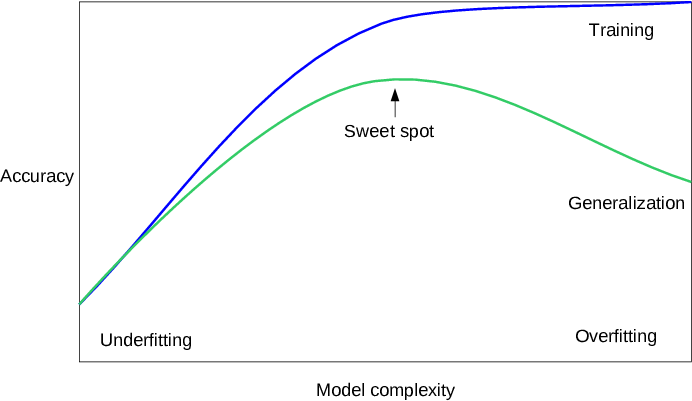
\includegraphics[scale=0.5]{../img/tradeoff_overfitting_underfitting.png}
	\caption{Trade-off tra overfitting e underfitting}
	\label{fig:tradeoff_img}
\end{figure}

% TODO: dal libro

\subsection{k-Nearest Neighbor}

Vediamo nello specifico uno dei più semplici algoritmi di ML: \emph{k-Nearest Neighbor} (k-NN). Questo è un algoritmo utilizzato sia per la classificazione che per la regressione. In entrambi i casi l'algoritmo si basa sul parametro $k$ fissato. Esso definisce il numero di vicini da prendere in considerazione per fare la predizione.


\begin{figure}[h!]
	\center
	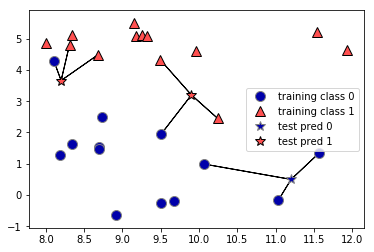
\includegraphics[scale=0.7]{../img/knn_classifier}
	\caption{Classificazione tramite k-NN di 3 elementi. Le stelle rosse rappresentano una classificazione rispetto alla classe 1 (dei triangoli) mentre le stelle blu rappresentano una classificazione rispetto alla classe 0 (dei cerchi).}
	\label{fig:knn_classifier}
\end{figure}

Supponiamo di avere due \emph{feature} (o caratteristiche), per semplicità, $ \mathrm{feature_0} $  e $ \mathrm{feature_1} $ le quale descriveranno -- insieme alla classe -- ogni record del nostro dataset.  Nel caso di classificazione tramite il k-NN in Figura \ref{fig:knn_classifier} è mostrato come un elemento non ancora etichettato venga classificato in base al tipo predominante dei suoi vicini. La scelta di $ k $ è quindi l'unica, ma fondamentale, scelta da prendere per determinare la precisione nella predizione dei futuri elementi.

\begin{figure}[h!]
	\center
	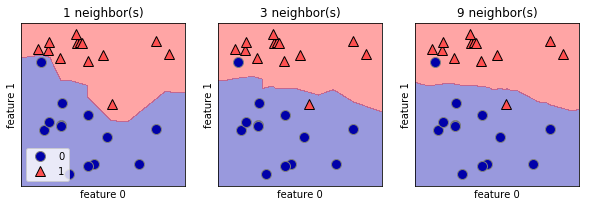
\includegraphics[scale=0.55]{../img/knn_comparison}
	\caption{Risultati di un classificatore k-NN, per diversi valori del parametro $k$ su un medesimo dataset. I cerchi e i triangoli indicano le osservazioni del dataset appartenenti a due classi, mentre le aree blu e rosse indicano gli esiti della classificazione.}
	\label{fig:knn_difference}
\end{figure}


In Figura \ref{fig:knn_difference} viene mostrato come influisce la scelta di differenti parametri $ k $ su uno stesso campione.

Questo algoritmo è spesso utilizzato con un $ k $ dispari per escludere casi di indecisione e quindi poter sempre definire la classe del nuovo dato.

Nel caso di regressione tramite il k-NN, il risultato sarà pari alla media dei valori target dei $ k $ più vicini.
\begin{figure}[h!]
	\center
	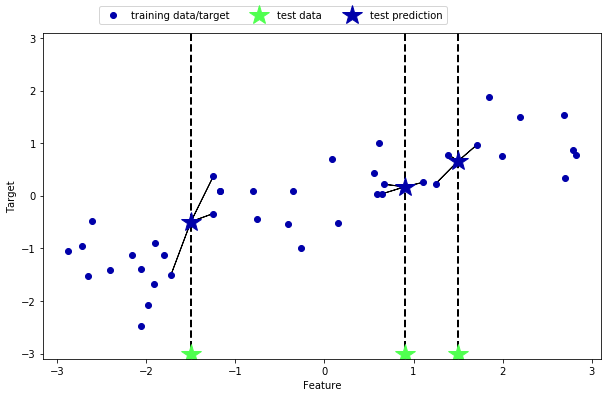
\includegraphics[scale=0.6]{../img/knn_regressor}
	\caption{Risultato di un regressore k-NN, per $k$ pari a 3. I cerchi indicano le osservazioni del dataset, le stelle verdi indicano il nuovo elemento da predire e le stelle blu gli esiti della predizione.}
	\label{fig:knn_regressor}
\end{figure}
Immaginiamo di avere, nel nostro dataset, due \emph{feature} per ogni elemento: $ \mathrm{Target} $ e $ \mathrm{Feature} $. $ \mathrm{Feature} $ rappresenta il valore su cui vogliamo basare il modello e $ \mathrm{Target} $ il valore che vogliamo predire. Prendendo ad esempio un $ k $ pari a 3 otteniamo (come vediamo in Figura \ref{fig:knn_regressor}) che il nuovo elemento da predire (la stella verde) avrà come valore $ \mathrm{Target} $ (la stella blu) la media dei $ \mathrm{Target} $ dei 3  elementi più vicini sull'asse delle ascisse (l'asse delle \emph{feature}).


\subsection{Modelli lineari}
I modelli lineari sono una classe di modelli che cercano di effettuare predizioni utilizzando una funzione lineare basata sull'insieme delle \emph{feature} dell'elemento da analizzare. 
Nel caso della regressione, la funzione di cui parliamo è definita come segue:
\[ y = w_{0}x_{0} + w_{1}x_{1} + ... + w_{n}x_{n} + b ,\]
dove $n$ è il numero di \emph{feature}, $x_{i}$ le \emph{feature}, $ w_{i} $ i pesi da attribuire a queste ultime e $ b $ un termine noto.
Prendendo una sola \emph{feature} (quindi $ n $ pari a 1), $ y $ risulterebbe:

\[ y = w_{0}x_{0} + b,\]
che è esattamente la funzione di una linea retta, dove $ w_{0}$ è il coefficiente angolare e $ b $ è lo scostamento dall'origine degli assi.

Riprendendo l'esempio precedente, supponiamo che si voglia quantificare il numero dei giorni necessari per guarire un paziente malato.
Supponiamo inoltre, per semplicità, di avere una sola caratteristica indicante l'età del paziente.
Nel grafico in Figura \ref{fig:linear_regression} è rappresentato il dataset dei pazienti le cui coordinate sono l'età sull'asse delle ascisse e i giorni di guarigione sull'asse delle ordinate.

È possibile tracciare una retta denominata retta di regressione che approssima tutti i punti definiti nel dataset. 

\begin{figure}[h!]
	\center
	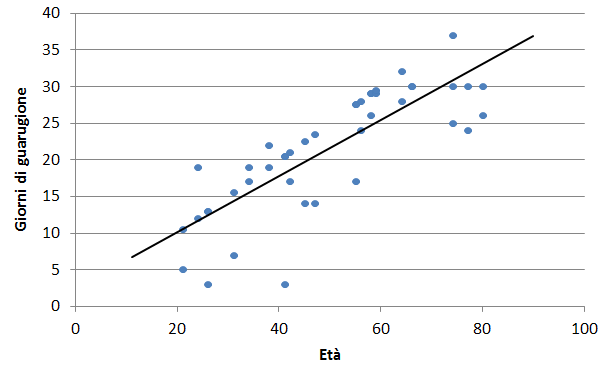
\includegraphics[scale=0.6]{../img/linear_regression}
	\caption{Regressione lineare. I punti rappresentano i pazienti e la retta nera rappresenta la retta di regressione che approssima meglio all'andamento di tutti i punti}
	\label{fig:linear_regression}
\end{figure}

I modelli lineare si possono applicare anche al contesto della classificazione, modificando leggermente la loro formulazione ovvero introducendo degli intervalli per definire a quale classe appartiene il singolo caso. Nella classificazione binaria ad esempio, la formula risulterebbe come segue:
\[ y = w_{0}x_{0} + w_{1}x_{1} + ... + w_{n}x_{n} + b > 0, \]
dove, supponendo di avere le classi $ \mathrm{C_1} $ e $ \mathrm{C_0} $, se la $ y $ fosse maggiore di $ 0 $, l'oggetto descritto dagli $x_{i}$ verrebbe classificato come $ \mathrm{C_1} $, altrimenti come $ \mathrm{C_0} $.
%
%Nella figura xxx è mostrato l'esempio appena citato, dove i cerchi sono la classe 0 e i triangoli la classe 1.

\subsection{Support Vector Machine}
Le Support Vector Machine (SVM) sono una classe di modelli che si occupa di individuare un iperpiano utile a separare i punti in uno spazio e quindi dividerli in diversi gruppi. 

Il primo problema che le SVM devono risolvere è capire quale sia l'iperpiano che suddivide nel modo ``migliore" i dati. 
%Per capire come l'algoritmo definisca ``migliore" un certo sistema di suddivisione.

\begin{figure}[h!]
	\center
	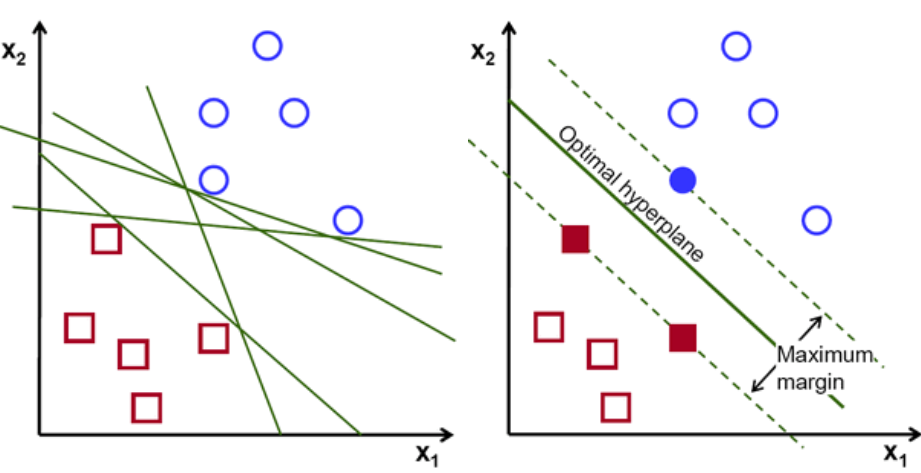
\includegraphics[scale=0.4]{../img/svc} %https://medium.com/@george.drakos62/support-vector-Machine-vs-logistic-regression-94cc2975433f
	\caption{Possibili iperpiani che dividono lo spazio (a sinistra) e iperpiano ``migliore" (a destra)}
	\label{fig:svc}
\end{figure}

Nel grafico di sinistra della Figura \ref{fig:svc} è possibile notare due gruppi distinti di punti (i cerchi blu e i quadrati rossi), che possono essere divisi dagli iperpiani raffigurati con linee verdi. Queste linee sono candidate ad essere i ``migliori" divisori per i due insiemi ma per decidere quale sia il migliore si considerano i punti P più vicini a ogni iperpiano I. Questi punti vengono definiti vettori di supporto (o \emph{support vector}). Per ogni iperpiano I e i relativi vettori di supporto V, viene calcolata la distanza tra I e V che viene chiamato ``margine". Si definisce quindi iperpiano migliore, l'iperpiano che riesce a massimizzare il margine dai rispettivi vettori di supporto. Nell'immagine destra in Figura \ref{fig:svc} mostra l'iperpiano ``migliore" ovvero l'iperpiano che massimizza il ``margine".

Nei casi reali capita spesso che lo spazio non è linearmente separabile. Per ovviare a questo problema si ricorre alle funzioni \emph{kernel} che sono in grado di mappare dei vettori da uno spazio $n$-dimensionale a uno spazio $m$-dimensionale.
Supponiamo il caso, rappresentato in Figura \ref{fig:svc_non_linear}, dove si hanno due sole dimensioni ma dove non è possibile suddividere i punti con una semplice linea.

\begin{figure}[h!]
	\center
	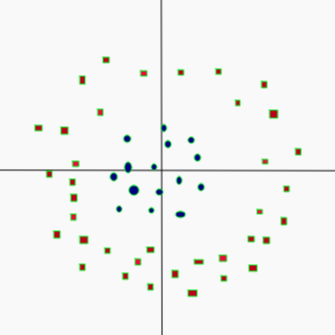
\includegraphics[scale=0.5]{../img/svc_non_linear} %https://medium.com/@george.drakos62/support-vector-Machine-vs-logistic-regression-94cc2975433f
	\caption{Dati non divisibili linearmente}
	\label{fig:svc_non_linear}
\end{figure}

Tramite una funzione \emph{kernel} trasformiamo i punti definiti dalle coordinate $x$ e $y$, in punti aventi coordinate $x$, $y$ e $z$. Questa trasformazione è conosciuta come trucco del \emph{kernel} (o \emph{kernel trick}). Essa permette di trasformare uno spazio $n$-dimensionale in uno spazio $m$-dimensionale, dove $m$ è spesso più grande di $n$. Così facendo possiamo rappresentare l'insieme in uno spazio tridimensionale e tracciare un iperpiano che suddivide in modo lineare i punti nello spazio, per poi ridefinirlo secondo le due dimensioni iniziali di partenza.
Aggiungiamo quindi una terza dimensione $z$ e definiamola come segue:
%Come esplicato in \cite{towards_data_science},
%TODO: refrenzia il post(https://towardsdatascience.com/https-medium-com-pupalerushikesh-svm-f4b42800e989), riporto l'esempio esplicativo:
%presi dei punti in uno spazio bidimensionale capita che questi non siano suddivisibili tramite una retta.

\[ z = x^2 + y^2.\]

Il risultato ottenuto è mostrato in Figura \ref{fig:svc_on_z_axis} e da esso si evince che si possono facilmente dividere i punti nelle due classi utilizzando una retta di equazione

\[ z = k ,\]
dove $k$ è una costante.

Quindi quando ci si trova davanti a problemi di suddivisione dell'iperspazio bisogna spesso ricorrere al trucco del \emph{kernel}. 

\begin{figure}[h!]
	\center
	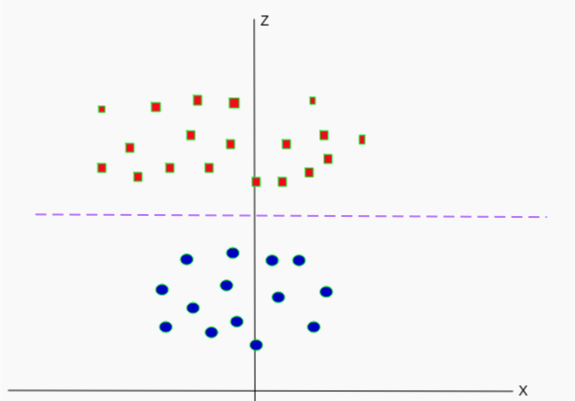
\includegraphics[scale=0.4]{../img/svc_on_z_axis} %https://medium.com/@george.drakos62/support-vector-Machine-vs-logistic-regression-94cc2975433f
	\caption{Dati visti sull'asse z}
	\label{fig:svc_on_z_axis}
\end{figure}

\pagebreak

%SVMQuesto trucco prevede anche dei parametri $ C $ e $ \gamma $, detti iperparametri (o parametri di tuning).
%Essi influiscono sulla selezione dell'iperpiano che si va ad ottenere nello spazio inziale:
%\begin{itemize}
%	\item $C$: è il parametro che consente di definire un costo nell'errore della suddivisione dei punti, vale a dire che nel caso in cui si scelga una C grande, ogni singolo errore avrà un costo elevato, andando cosi ad adattare il modello SVM nel modo più preciso possibile al training set. Adattando il modello in maniera eccessiva al training set, però, si rischierebbe di andare in overfitting e quindi comporterebbe ad una classificazione errata nel caso di esempi estranei all'insieme dei dati di allenamento. Avendo invece, una C piccola, il costo di errore sarà basso, il quale comporterà che durante l'allenamento del modello, saranno presenti diversi errori di classificazione, però, così facendo si sta generalizzando maggiormente il modello a nuovi casi da etichettare, il che può essere positivo. Vi rimando alla figura \ref{fig:tradeoff_img} che denota un buon livello di accuratezza, il quale sta a metà tra overfitting e underfitting.
	
%	\item $\gamma$: questo parametro definisce fino a che punto arriva l'influenza di un singolo esempio di allenamento. Se ha ha un valore molto elevato, allora il limite della decisione dipenderà solo dai punti molto vicini alla linea, il che si traduce effettivamente nell'ignorare alcuni dei punti che sono molto lontani dal limite della decisione. Questo perché i punti più vicini ottengono più peso e si traduce in una curva ondulata come mostrato nel grafico precedente. D'altra parte, se il valore gamma è basso anche i punti più lontani ottengono un peso considerevole e otteniamo una curva più lineare.
%\end{itemize}

\subsection{Alberi di decisione}

Gli alberi di decisione, o \emph{decision trees} (DT) sono dei modelli di classificazione o di regressione la cui logica si basa su una struttura ad albero. I nodi dell'albero rappresentano delle domande (o \emph{test}) la cui risposta è di tipo binario (vero o falso) mentre le foglie rappresentano le classi che vogliamo predire.
\begin{figure}[h!]
	\center
	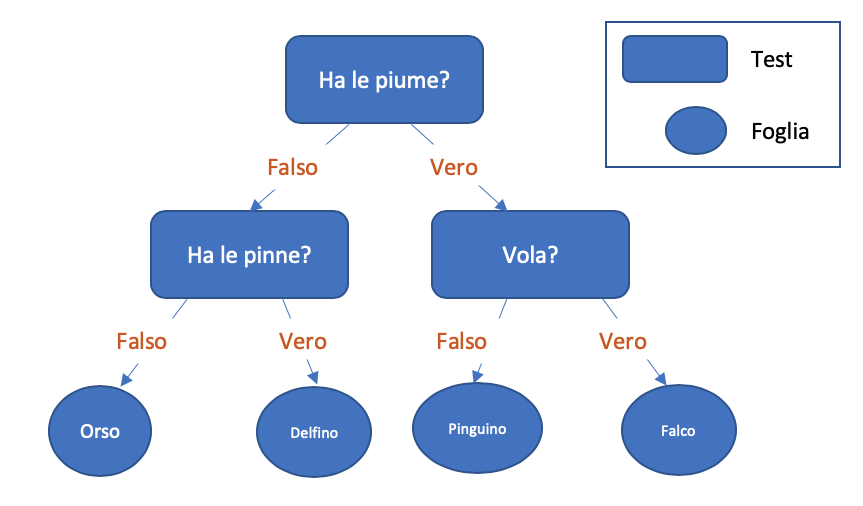
\includegraphics[scale=0.35]{../img/example_decision_tree} %https://medium.com/@george.drakos62/support-vector-Machine-vs-logistic-regression-94cc2975433f
	\caption{Esempio di albero di decisione per la classificazione di un animale}
	\label{fig:example_decision_tree}
\end{figure}
%L'algoritmo predispone delle domande sulla base dei dati contenuti nell'input. 

\noindent{Supponiamo, ad esempio, di voler distinguere un animale tra: falco, pinguino, delfino e orso. Nell'esempio in Figura \ref{fig:example_decision_tree} l'algoritmo parte dalla domanda D: ``Ha le piume?". In questo modo abbiamo definito il primo nodo N dell'albero rappresentato da D. Sapendo che i \emph{test} previsti dall'algoritmo restituiscono un output binario, da N si diramano due sotto-alberi, rappresentati dalle categorie $ \mathrm{C_0} $(``ha le piume") e $ \mathrm{C_1} $(``non ha le piume"). Considerando gli elementi appartenenti a $ \mathrm{C_1} $ (orso e delfino), mediante un'ulteriore domanda si possono distinguere i due animali e quindi determinare la classe di appartenenza di ciascuno di essi. Seguendo quindi la domanda ``Ha le pinne?", se la risposta è si, si sta parlando del delfino, ovvero l'unico animale tra i quattro che non ha le piume e ha le pinne, altrimenti deve trattarsi dell'orso. Seguendo questa logica è possibile arrivare -- con le giuste domande -- a fare delle predizioni.}

Questo è un esempio eccessivamente semplificato. Nella realtà i dati che vengono analizzati hanno spesso valori di tipo continuo, quindi il \emph{test} è del tipo: ``$ x $ è maggiore di $ k $?", dove $x$  rappresenta una \emph{feature} del dataset e $k$ rappresenta una costante.

Una volta definiti i \emph{test} è possibile suddividere lo spazio su cui rappresentiamo i dati in diverse aree, ognuna delle quali è rappresentata da una foglia (e quindi da una classe).


\begin{figure}[h!]
	\center
	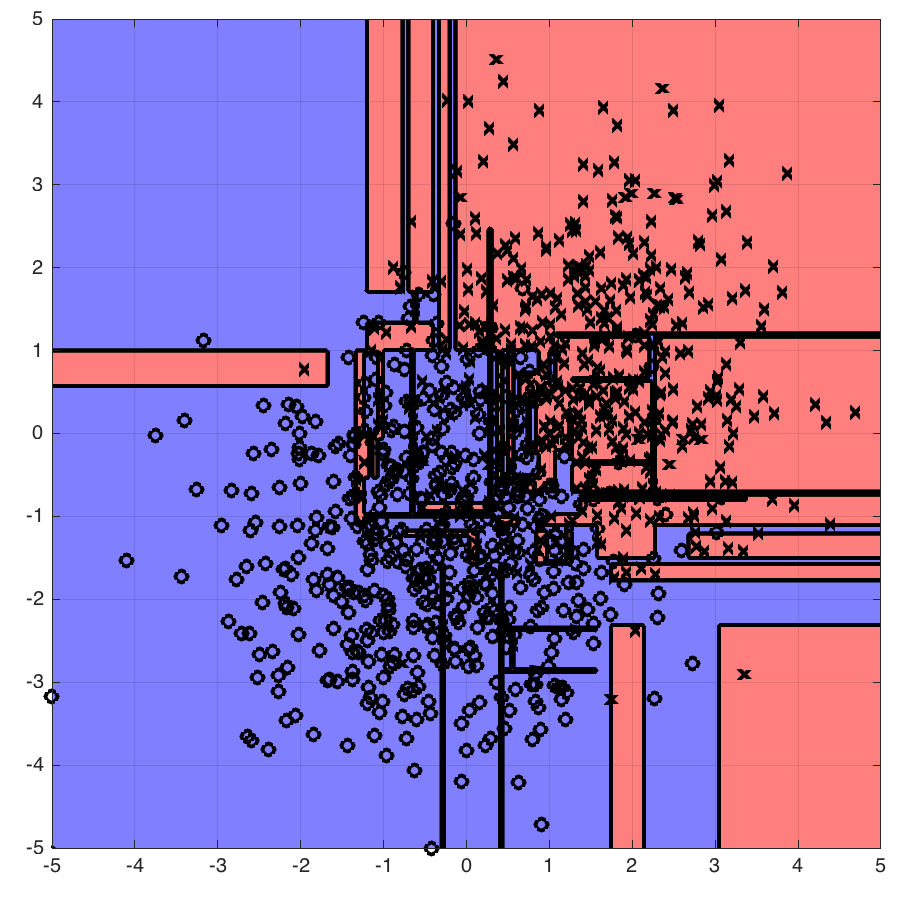
\includegraphics[scale=0.2]{../img/overfit_decision_trees1} %https://medium.com/@george.drakos62/support-vector-Machine-vs-logistic-regression-94cc2975433f
	\caption{Overfitting dei dati con l'albero di decisione}
	\label{fig:overfit_decision_trees1}
\end{figure}

Come abbiamo già visto negli altri algoritmi, il problema dell'\emph{overfitting} e \emph{underfitting} sono problemi ricorrenti che si presentano anche nel caso degli alberi di decisione.
Infatti se viene costruito un albero troppo dettagliato, e quindi con un elevato livello di profondità, il modello tende ad adattarsi in maniera eccessiva ai dati usati in fase di allenamento generando un problema di \emph{overfitting}. In Figura \ref{fig:overfit_decision_trees1} è raffigurato un albero di decisione evidenziando le aree che corrispondono alle sue foglie su un piano bidimensionale. Nella figura è possibile osservare zone blu e rosse eccessivamente piccole le quali sono sintomo di un elevato livello di dettaglio nelle domande. Siamo quindi in presenza di un problema di \emph{overfitting}.

Analizzando un caso simile è possibile vedere tramite il grafico riportato in Figura \ref{fig:overfit_decision_trees2} come l'errore su un insieme di dati non incluso in quello di allenamento cresce con l'aumentare della profondità. Il grafico mostra che più permettiamo all'albero di avere tanti livelli, più lui ha la capacità di adattarsi meglio ai dati di training, e a partire da una certa lunghezza inizia a farlo a detrimento della sua capacità di generalizzazione. Questo succede proprio perché il modello si è adattato in maniera eccessiva all'insieme di dati di allenamento.
\begin{figure}[h!]
	\center
	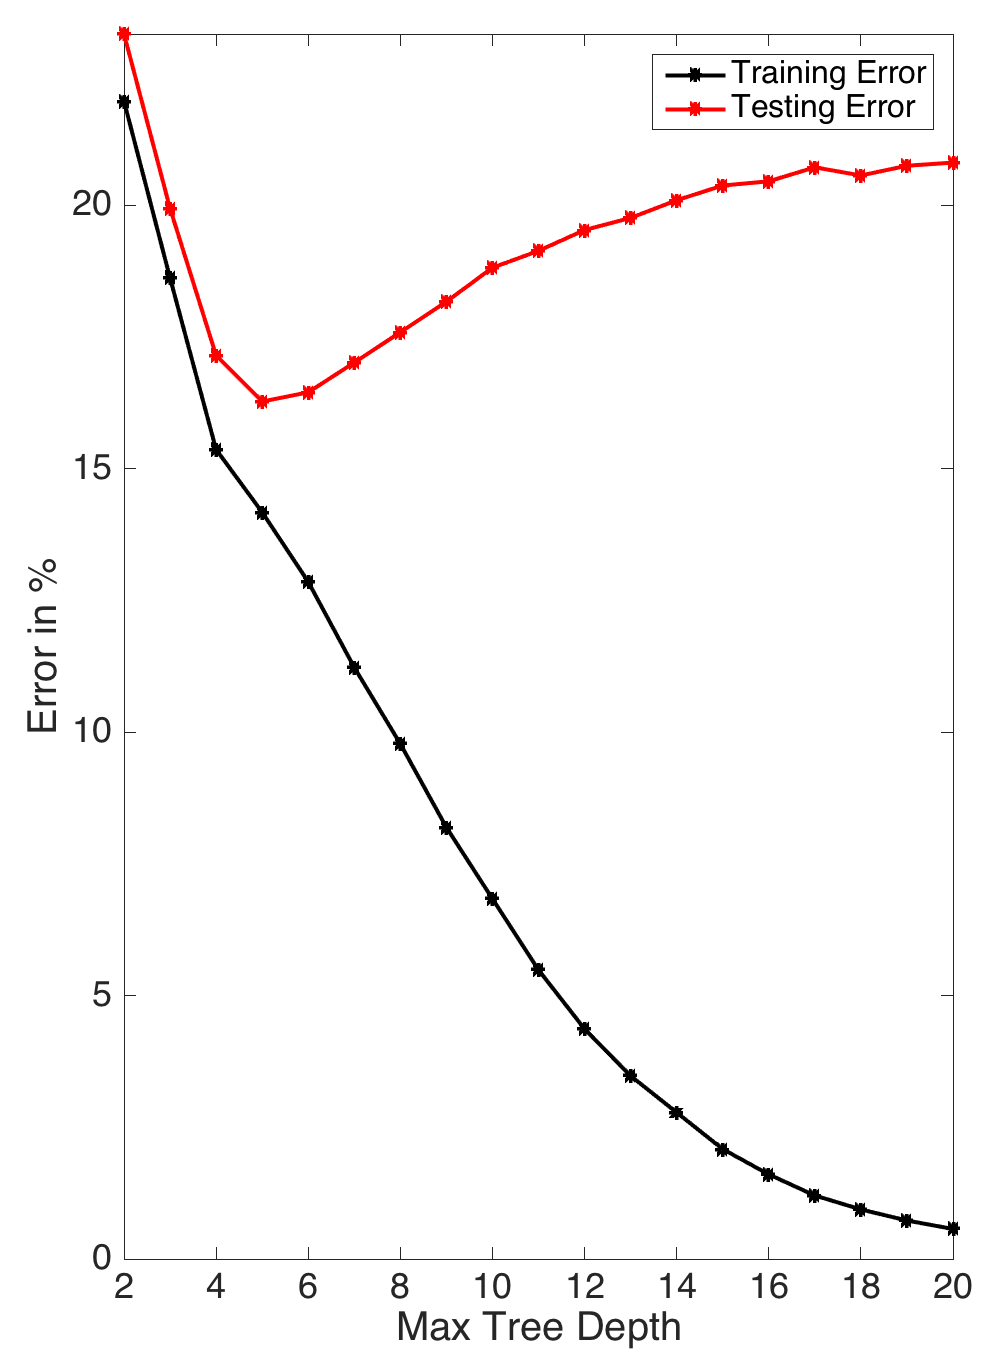
\includegraphics[scale=0.18]{../img/overfit_decision_trees2} %https://medium.com/@george.drakos62/support-vector-Machine-vs-logistic-regression-94cc2975433f
	\caption{Grafico di \emph{overfitting} per diversi alberi di decisione in cui ogni punto corrisponde ad un modello DT la cui profondità è definita sull'asse delle ascisse. La curva nera rappresenta l'errore di precisione nella predizione di dati di allenamento mentre la curva rossa rappresenta l'errore sui dati di test. }
	\label{fig:overfit_decision_trees2}
\end{figure}

Per risolvere questo problema esistono due strategie:
\begin{itemize}
	\item far terminare lo sviluppo dell'albero dopo pochi passi (pre-potatura) ovvero limitare a priori la profondità dell'albero,
	
	\item rimuovere i nodi che contengono informazioni poco significative (post-potatura).
\end{itemize}

\section{Non supervisionato}
La tecnica non supervisionata (o \emph{unsupervised learning}) è il secondo importante approccio all'applicazione del ML. Cosa si intende dire con ``non supervisionata"? Come può una macchina imparare se nessuno la guida nella scelta delle decisioni?
Questa è proprio la sfida che si vuole superare con questa tecnica, ovvero far estrapolare al calcolatore delle informazioni ``nascoste" all'interno dei dati che gli vengono forniti. Queste informazioni solitamente sono legami, schemi o regole che i dati tendono a seguire.

Ci sono diversi utilizzi di ML non supervisionato, in questa sezione ci limiteremo a elencarne alcuni. Il principale algoritmo di \emph{Unsupervised Learning} è il clustering, ossia una tecnica in grado di suddividere in gruppi distinti elementi che hanno dati e caratteristiche in comune.

Supponiamo di aver scattato una serie di fotografie in cui sono raffigurate delle persone e decidiamo di caricarle su un social network. Supponiamo inoltre che durante il caricamento il social network su cui le stiamo caricando visiona le foto e applichi proprio un algoritmo di clustering. In che modo? L'algoritmo non sa né chi siano le persone raffigurate né quante siano. Andrà, però, a cercare tutti i volti nelle fotografie che abbiamo caricato e, successivamente, dopo aver definito una lista di tutti i volti presenti in ogni foto, tramite un algoritmo di clustering cercherà delle somiglianze in questi volti. Alla fine della sua esecuzione l'algoritmo avrà raggruppato le foto dove è presente lo stesso soggetto.

Un altro esempio di utilizzo ricade nell'ambito della sicurezza informatica. Al giorno d'oggi i tipi di attacco conosciuti sono probabilmente solo la punta dell'iceberg. Ricorrendo, però, a tecniche di clustering possiamo riuscire a individuare e bloccare attacchi tuttora sconosciuti. 
Supponiamo di essere collegati al sito della nostra banca che memorizza tutte le operazioni che facciamo. Supponiamo inoltre, di effettuare quotidianamente delle specifiche operazioni all'incirca alla stessa ora, collegandoci da una determinata località geografica. Tramite il ML non superivsionato queste informazioni potrebbero essere utilizzate per creare dei cluster, che ci individuino sulla base delle nostre operazioni.
%Tramite il ML non supervisionato il sistema memorizzerà tutte le operazioni che faremo. Supponiamo di effettuare quotidianamente delle specifiche operazioni ad un fissato orario, in una determinata località geografica. Bene, queste informazioni vengono salvate dal calcolatore il quale le utilizzerà per creare dei cluster, ossia per riconoscerci sulla base delle nostre operazioni ricorrenti tramite orario, località geografica e altre possibili informazioni.
Supponiamo ora che un malintenzionato, dall'altra parte del mondo, a un orario differente da quello a noi abituale, riesca ad accedere al nostro profilo bancario. L'algoritmo sarebbe in grado di notare che è in atto qualcosa di anomalo. Nonostante nessuno abbia specificato al calcolatore quali sono le operazioni abituali effettuate dell'utente, il calcolatore, mediante tecniche di clustering, è in grado di riconoscere le operazioni abituali e mandare un messaggio di allarme se individua possibili casi anomali.

\section{Semi-supervisionato}

L'approccio semi-supervisionato (o \emph{semi-supervised}), non è un vero e proprio approccio, bensì una tecnica che sta a metà tra le due appena viste: supervisionato e non supervisionato. Questo approccio consiste nel combinare le due tecniche e fornire un risultato basandosi su un input eterogeneo costituito da dati etichettati e dati non etichettati.

Questo metodo risulta utile quando si ha una grande mole di dati che vengono etichettati manualmente da utenti specializzati. Nella situazione reale non sempre questo è possibile, proprio perché possono mancare risorse umane competenti o tempistiche adeguate per etichettare tutti i dati. Esistono differenti algoritmi per l'apprendimento automatico mediante un sistema semi-supervisionato:
\begin{itemize}
	\item \emph{self training},
	\item \emph{multi-view training},
	\item \emph{self-ensembling}.
\end{itemize}

Per quanto riguarda il \emph{multi-view training}, possiamo dire che esso mira a formare diversi modelli con diverse visualizzazioni dei dati. Idealmente queste viste sono complementari e i modelli possono collaborare per migliorare il risultato finale. Queste viste possono differire in diversi modi, ad esempio possono differire nelle funzionalità che utilizzano, nelle architetture dei modelli o nei dati su cui i modelli vengono formati.

Il \emph{self-ensembling}, come il \emph{multi-view training}, punta a combinare diverse varianti dei modelli. A differenza di quest'ultimo, però, la diversità nei modelli non è un punto chiave perché il \emph{self-ensembling} utilizza principalmente un singolo modello in diverse configurazioni al fine di rendere più affidabili le previsioni del modello finale. 

Vediamo ora più in dettaglio l'algoritmo di \emph{self training} che è stato uno dei primi algoritmi a essere sviluppato ed è l'esempio più diretto di come le previsioni di un modello possono essere incorporate nel training del modello.

L'algoritmo di \emph{self training} prevede, quindi, di basarsi per quanto possibile su dati che sono stati preventivamente etichettati, avendo anche a disposizione dati non etichettati. Questi ultimi vengono comunque utilizzati, ma in maniera più cauta. Prima di allenare il modello l'algoritmo si concentrerà ad etichettare gli input non ancora etichettati.

Come viene spiegato nell'articolo \cite{ruder} %[https://ruder.io/semi-supervised/], 
la logica di classificazione dei dati non ancora classificati segue quanto scritto: ``Formalmente, l'auto-etichettamento avviene su un modello $ M $ avente un insieme $ L $ di dati di allenamento etichettati con delle etichette contenute in $ C $ e un insieme non etichettato $ U $. A ogni iterazione, per ogni $x \in U$, il modello fornisce delle predizioni su $ x $ sotto forma di probabilità $ p(x, c) $ ovvero la probabilità che $ x $ appartenga alla classe $ c $ per ogni $ c \in C $. Tra le probabilità appena calcolate, definiamo $ P(x, c) $ come la probabilità avente il valore maggiore, allora se $ P $ è più grande di una soglia $ T $, $ x $ verrà aggiunto a $ L $ con l'etichetta $ c $. Questo processo viene ripetuto per un numero fisso di iterazioni o fino a quando non ci sono più dati da etichettare.". \cite{ruder} %TODO: \footnote{traduzione libera del testo}

Nel pseudo-codice \ref{algo:self_training} è esplicitato quanto detto sopra:
\begin{algorithm}
	\caption{self-training}\label{algo:self_training}
	\begin{algorithmic}[1]
		\Repeat
		\State $m \gets train\_model(L)$
		\For {$x \in U$}
		\If {$\max m(x) > \tau$}
		\State $L \gets L \cup \{(x, p(x))\}$
		\EndIf
		\EndFor
		\Until {no more predictions are confident}
	\end{algorithmic}
\end{algorithm}

\section{Apprendimento con rinforzo}
Il quarto e ultimo approccio è chiamato apprendimento con rinforzo, o reinforcement learning (RL), e si differenzia da quelli visti fino ad ora. Questo paradigma si occupa di problemi di decisione sequenziali, in cui l'azione da compiere dipende dallo stato attuale del sistema e ne determina quello futuro. In altre parole, questo è un sistema dinamico che può apprendere in seguito a ogni decisione presa, a prescindere che questa sia giusta o sbagliata.

\begin{figure}[h!]
	\noindent
	\center
	\label{fig:rl_scenario}
	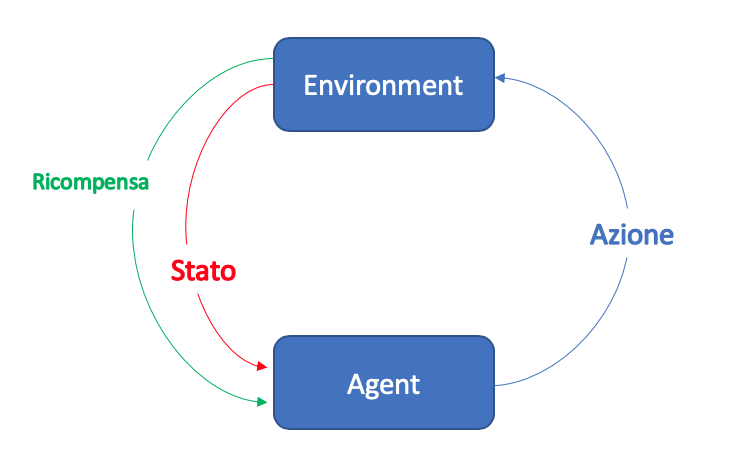
\includegraphics[scale=0.35]{../img/rl_scenario}
	\caption{Scenario RL: l'Agent compie un'azione in un Environemnt che porta a un cambiamento di stato e a una ricompensa che influenzeranno le future scelte dell'Agent}
\end{figure}

% (https://www.aitrends.com/education/udacitys-school-of-ai-opens-the-new-deep-reinforcement-Learning-nanodegree-program-for-enrollment/) (https://www.guru99.com/reinforcement-Learning-tutorial.html)

Quando il sistema prende una decisione otterrà successivamente una ``ricompensa" sotto forma di punteggio che sarà alto o basso a seconda che la decisione presa sia giusta o sbagliata. Con questa logica la macchina cercherà di fare sempre meglio per arrivare a ottenere il punteggio più alto possibile prendendo, così, solo le decisioni corrette. 

\section{Riduzione della dimensionalità}

Nel ML, come abbiamo visto, l'input gioca un ruolo fondamentale nello sviluppo di un modello che riesca a predire nel modo corretto i nuovi dati che verranno esaminati da quest'ultimo.
In questo lavoro ci concentreremo proprio sul riconoscimento dei volti all'interno delle immagini, quindi, per parlare dell'importanza del ridimensionamento delle \emph{feature}, faremo riferimento proprio all'analisi di immagini che raffigurano persone, animali o oggetti.

Spesso ci troviamo di fronte a dati di dimensioni eccessive che comportano, \emph{in primis}, dei problemi a livello tempistico e poi anche a livello computazionale. Ci basti pensare che quando cerchiamo di analizzare un'immagine per estrapolarne delle informazioni (riconoscimento di oggetti, persone, animali) dobbiamo passare in rassegna tutti i pixel! Supponiamo di prendere un'immagine a bassa risoluzione, ad esempio 500x500, ciò significherebbe trovarsi davanti a $ 500^2 $ pixel, ovvero 250.000 elementi per una singola immagine! Questo comporterebbe, quindi, analizzare uno spazio sovra dimensionato, con appunto 250.000 dimensioni.

Considerare uno spazio di quelle dimensioni è impensabile, proprio per questo ci vengono in soccorso delle tecniche che si occupano di ridurre il numero di elementi che definiscono l'oggetto estrapolandone solamente le informazioni più utili, informazioni che permettono di differenziare un oggetto da un'altro.

Pensiamo ad esempio a un'immagine in cui è raffigurato il volto di una persona. E' normale pensare che non tutti i pixel siano di fondamentale importanza per riconoscere il soggetto raffigurato. Ad esempio, tutti i pixel presenti nei bordi dell'immagine saranno sicuramente da scartare in quanto non ci diranno niente sulla persona raffigurata, così come molti altri pixel che raffigurano parti poco interessanti, come lo sfondo dell'immagine. Vediamo nei due paragrafi seguenti quali sono gli strumenti più utilizzati per risolvere questo tipo di problemi.


\subsection{Analisi delle componenti principali}
L'analisi delle componenti principali o \emph{Principal Component Analysis} (PCA) è un metodo di riduzione della dimensionalità. Lo scopo di PCA è quello di diminuire il numero di informazioni necessarie a descrivere un'osservazione limitando il più possibile la perdita di informazioni. 

Consideriamo la matrice A in cui le colonne rappresentano le \emph{feature} e le righe le osservazioni. In primo luogo, viene calcolata la media per ogni colonna della matrice A. Una volta calcolato il vettore risultante (la media) lo faremo coincidere con l'origine degli assi, in questo modo ogni punto verrà traslato di conseguenza. Successivamente calcoliamo la matrice di covarianza per A, la quale servirà per calcolare gli autovalori. Una volta ottenuto l'autovalore a questo punto viene calcolato l'autovettore il quale identifica la retta che meglio si adatta a tutti i punti, ovvero la retta R che minimizza la somma delle distanze dei punti da R. Questa viene chiamata $\mathrm{PC_1}$. Si ripete questo passaggio per ogni dimensione, mantenendo la perpendicolarità della nuova retta (o $\mathrm{PC_{n}}$) rispetto all'ultima retta calcolata (o $\mathrm{PC_{n-1}}$). 
Una volta calcolate tutte le \emph{principal component} dello spazio PCA, per ognuna di esse si utilizzerà l'autovettore per determinare la nuova posizione di ogni punto scalandolo sul rispettivo asse. Una volta scalati tutti i punti si calcola la varianza per ogni asse. Il valore della varianza $\sigma^2$ rispetto al i-esimo $\mathrm{PC_{i}}$, calcolata in percentuale, ci dice quanto pesa l'informazione contenuta sulla dimensione $i$. Questo ci permetterà quindi, di eliminare gli assi meno interessanti, ovvero gli assi con la varianza in percentuale più bassa. La stessa informazione è di fatto contenuta negli autovalori calcolati precedentemente. 

Questa tecnica, oltre a semplificare il lavoro di manipolazione delle \emph{feature}, aiuta a migliorare i risultati degli algoritmo di ML poiché estrapola le informazioni realmente utili per predire la classe o il valore da attribuire ad un oggetto. Tutte le informazioni di contorno, come ad esempio i pixel situati sul bordo di un'immagine, possono essere fuorvianti per l'algoritmo di apprendimento. Questo è il motivo per cui la tecnica PCA semplifica e ottimizza i valori risultanti ed è ampiamente utilizzato nell'ambito di:
\begin{itemize}
	\item riconoscimento facciale \cite{3d_face_recocgnition_pca},
	\item image compression \cite{image_compression_pca},
	\item rilevamento di pattern in campi ad alta dimensionalità \cite{pattern_recocgnition_pca},
	\item data mining \cite{data_mining_pca}.
\end{itemize}

\subsection{t-Distributed stochastic neighbor embedding}
%Documenta con delle immagini prendedole dal video https://www.youtube.com/watch?v=NEaUSP4YerM
\emph{t-Distributed stochastic neighbor embedding} (t-SNE) è una tecnica di riduzione della dimensionalità non lineare che si presta particolarmente alla mappatura di spazi ad alta dimensionalità riducendoli in uno spazio a minori dimensioni. L'algoritmo modella i punti in modo che oggetti vicini nello spazio originale risultino vicini nello spazio a dimensionalità ridotta e analogamente oggetti lontani nello spazio originale risultino lontani nello spazio a dimensionalità ridotta.

Per spiegare il funzionamento di questo algoritmo basiamoci su un caso semplice: un set bidimensionale $S$ di dati. Con questo esempio spieghiamo quindi il funzionamento di t-SNE e come è possibile passare da due dimensioni ad una sola, trasformando coerentemente le distanze tra i punti osservati. Per farlo ci basiamo, inoltre, sulle probabilità che un elemento sia vicino ad un'altro. Per ogni punto $ x $ centriamo su di esso una curva gaussiana e inseriamo ogni altro punto $ y \neq x $ 
sotto la distribuzione gaussiana centrata in $ x $, per poi calcolarne la densità di probabilità (o \emph{score}).
%la quale verrà utilizzata per calcolare la probabilità che ogni altro elemento, sia vicino a x. 

Viene utilizzata la curva gaussiana perché lavora bene su casi come questo: restituisce un valore elevato se un elemento è molto vicino a $x$ e una valore molto basso se questo è lontano da $x$. A questo punto normalizziamo la curva per tutti i punti in modo che essi abbiano una misura proporzionata e non indipendente. La distribuzione può in realtà essere manipolata tramite una variabile denominata `perplessità' (o \emph{perplexity}), la quale modifica la varianza e quindi l'ampiezza della curva.
In questo modo otteniamo la matrice quadrata $ M_{1} $ con tutti gli \emph{score} per ogni coppia. Ora inseriamo tutti i punti in maniera casuale su un'unico asse. Analogamente all'utilizzo che abbiamo fatto della curva gaussiana calcoliamo la probabilità di vicinanza tra i punti, con la differenza che questa volta useremo la distribuzione t di Student (in inglese Student t distribution, da cui deriva la t di t-SNE). Otteniamo così una seconda matrice quadrata $ M_{2} $, la quale sarà, probabilmente, molto diversa da $ M_{1} $. L'obiettivo adesso è quello di adattare la matrice $ M_{2} $ a $ M_{1} $ in modo che le distribuzioni di probabilità che descrivono i dati nello spazio ad alta dimensionalità e a bassa dimensionalità siano il più ``vicini" possibili minimizzando la pseudo-distanza (anche detta ``divergenza di Kullback-Leibler") tra queste. In questo modo siamo riusciti ad ottenere i cluster, visualizzabili nel grafico bidimensionale, in uno spazio monodimensionale.

Nella seconda parte dell'algoritmo, viene usata una t-distribution perché separa meglio i cluster nel piano generato. Se avessimo usato una distribuzione gaussiana, come nella prima parte, il risultato ottenuto sarebbe stato meno visibile, in quanto tutti i cluster si sarebbero ammassati al centro.

Questo è un esempio piuttosto semplice, ma nella realtà si possono adattare spazi a $n$ dimensioni con $ n \gg 2 $ a spazi molto inferiori a $n$. Nel Capitolo 3 utilizzeremo t-SNE per passare da uno spazio di dimensioni elevate a uno spazio bidimensionale o al più a 5 dimensioni. Vedremo quindi, utilizzando questo algoritmo, quali sono le prestazioni che riesce a fornire nel caso del riconoscimento facciale e di classificazione dei soggetti.
% 
%			CAPITOLO 2: Induzione di insiemi fuzzy
% 


\chapter{Induzione di insiemi fuzzy}
\label{ch:prova}

\section{La logica fuzzy}
La logica fuzzy (in italiano, logica sfocata), è un'estensione della logica booleana. Nella matematica booleana sono presenti solo due valori attribuili alle variabili: \emph{vero} e \emph{falso}. 
La logica fuzzy si definisce estensione della logica di Boole in quanto, al posto di prevedere solamente due possibili valori, viene previsto un insieme di valori continui compresi nell'intervallo [0, 1]. In questo intervallo, $0$ corrisponde al valore \emph{falso} e $1$ al valore \emph{vero}. Con questa estensione, oltre a poter dire \emph{vero} o \emph{falso} è possibile dire, tramite il grado di verità, quanto è vera una proprietà.
Quindi, data una proprietà \emph{P} e un elemento \emph{x}, si può dire:

\begin{center}
	\centering
	{

		\em{x rispetta P con valore y}
		
	}
\end{center} 
dove \emph{y} è compreso nell'intervallo $ [0,1] $.

Per fare un esempio più concreto si può pensare a tutte quelle cose che sono determinate in modo netto, in cui non esiste solo bianco o nero, bensì ci sono delle vie di mezzo più o meno vere.
Supponiamo di prendere un oggetto di cui diciamo ``essere freddo". Allora si può dire per esempio che:
\begin{itemize}
	\item un gelato ``è freddo" con valore (o grado di verità) uguale a 0.9,
	\item un bicchiere d'acqua a temperatura ambiente ``è freddo" con valore uguale a $ 0.4 $,
	\item la resistenza di una lampadina accesa ``è fredda" con valore uguale a 0.1.
\end{itemize}


\section{Gli insiemi fuzzy}
La logica fuzzy è strettamente legata alla matematica degli insiemi. Gli insiemi fuzzy sono un'estensione della teoria classica degli insiemi, secondo la quale un elemento appartiene o meno ad un insieme. %Con questa estensione, analogamente al grado di verità per la logica fuzzy, si definisce con
La teoria degli insiemi fuzzy è di fatto un'estensione della classica teoria degli insiemi con la differenza che questa, utilizza la logica fuzzy per valutare il valore di verità della proposizione "l'elemento x appartiene all'insieme A". Tale valore di verità prende il nome di grado di appartenenza dell'elemento all'insieme.
Il grado di appartenenza degli insiemi fuzzy $x \in [0,1]$ definisce quindi il grado di appartenenza ad un insieme. Per $ x $ pari a $ 1 $ l'elemento è, con un'alta probabilità, incluso nell'insieme, per $ x $ pari a $ 0 $ l'elemento è, al contrario, con una molta bassa probabilità, incluso nell'insieme, per tutti i valori compresi tra 0 e 1 l'appartenenza può essere più o meno forte.

Per fare un esempio definiamo lo spazio $ U $ come l'universo delle persone e un'insieme $ A $ che include tutte le persone giovani.
Per ognuna delle seguenti categorie di persone in $ U $:
\begin{itemize}
	\item neonato
	\item ventenne
	\item ottantenne
\end{itemize}
si può definire per ognuna di esse un grado di appartenenza all'insieme $ A $. Ad esempio:
\begin{itemize}
	\item neonato appartiene ad $ A $ con un valore pari a 1
	\item ventenne appartiene ad $ A $ con un valore pari a 0.8
	\item ottantenne appartiene ad $ A $ con un valore pari a 0.1
\end{itemize}
Formalizzando quanto appena detto, definiamo
% si può definire una funzione del grado di appartenenza nu basata su un predicato p in uno spazio U tale che:
\[ \mu_{A}: U \rightarrow [0,1] \]
dove $ \mu_{A} $ rappresenta una funzione, denominata funzione di appartenenza, che definisce il grado di appartenenza ad $ A $ per ogni elemento nell'universo dell'insieme $ U $. Un insieme fuzzy è definito dalle coppie ($x$,  $ \mu_{A}(x)$), quindi dall'elemento $ x $ e il relativo grado di appartenenza ad $ A $. Formalmente:
\[ A = \{  (x, \mu_{A}(x)) \mid x \in U\}. \]

\section{Fuzzylearn}

Nel capitolo precedente abbiamo visto le diverse tecniche utilizzate nel ML. L'algoritmo che andremo a descrivere, denominato \emph{fuzzylearn}\cite{fuzzylearn}, si basa sull'induzione di insiemi fuzzy e ricade nell'approccio supervisionato, ovvero quella tecnica che necessita di dati preventivamente valutati per effettuare predizioni.

In questo caso per predizione si intende il grado di appartenenza a un certo insieme fuzzy. 
%TODO fai un esempio
%TODO definisci prima possibilearn
%TODO citazione del testo del professore
Fissato un insieme fuzzy A, e dati due insiemi $ X = \{x_1, ..., x_n\} $ di valori nell'universo di A e $ M = \{\mu_1, ..., \mu_n\} $ dei corrispondenti gradi di appartenenza ad A, l'obiettivo di \emph{fuzzylearn}  consiste nel determinare un'approssimazione di A, e in particolare della sua funzione di appartenenza, partendo dai valori contenuti in $ X $ e $ M $.

%TODO: sistema indentazione
L'algoritmo \emph{fuzzylearn} si basa sulla risoluzione di due problemi:
\begin{itemize}
	\item determinare il sottoinsieme dell'universo in cui la funzione di appartenenza all'insieme fuzzy assume valore unitario,
	\item definire il comportamento della funzione di appartenenza nei casi rimanenti.
\end{itemize}

\subsection {Calcolo dell'insieme fuzzy}
Fissato un generico insieme fuzzy A, l'algoritmo \emph{fuzzylearn} si basa sulle ipotesi descritte di seguito:
\begin{itemize}
	\item Definiamo il core di A come l'insieme (classico) di tutti gli elementi dell'universo in corrispondenza dei quali il grado di appartenenza ad A è uguale a 1. Formalmente:
	\begin{center}
		\centering {
		$ c(A) = \{x \in U \mid \mu_A(x) = 1 \}. $
		}
	\end{center}
	Il core di A si può approssimare come l'insieme degli elementi di U le cui immagini tramite una funzione $ \phi $: $ U \mapsto H $ sono incluse in una ipersfera.
	
	\item Indicato con $ a $ il centro dell'ipersfera descritta nel punto precedente, il grado di appartenenza $ \mu_A(x) $ dipenderà solo dalla distanza di $ \phi(x) $ da $ a $.
\end{itemize}

Fatte queste ipotesi è possibile definire il seguente problema:
trovare la più piccola ipersfera avente centro $a$ e raggio $R$ che include la maggior parte delle immagini tramite $ \phi $ degli elementi $ x \in X $. Viste le ipotesi precedenti, per tutti i punti $ x $ mappati in questa ipersfera varrà dunque $ \mu_A(x) = 1 $. La formulazione matematica di questo problema determina un problema di ottimizzazione vincolata, la cui funzione obiettivo è
\[ \min R^2 + C\sum_{i=1}^{n} (\xi_{i} + \tau_{i}), \]
%R 2 + C (ξ i + τ i )
dove $ C $ è una costante di cui parleremo successivamente, mentre $ \xi $ e $ \tau $ sono le variabili di scarto utilizzate nel problema di ottimizzazione. $ \xi $ è la variabile slack legata al posizionamento dei punti all'interno dell'ipersfera mentre $ \tau $ è riferita al posizionamento dei punti all'esterno dell'ipersfera.

Alla funzione obiettivo descritta sopra aggiungiamo i seguenti vincoli:
\begin{equation}
\label{eq:1}
\begin{aligned}
\quad \mu_{i} \lVert \phi(x_{i}) - a \rVert ^2 \leq \mu_{i} R^2 + \xi_{i}\\
\end{aligned},
\end{equation}
\begin{equation}
\label{eq:2}
\begin{aligned}
\quad (1 - \mu_{i}) \lVert \phi(x_{i}) - a \rVert ^2 \geq (1 - \mu_{i})R^2 - \tau_{i} \\
\end{aligned},
\end{equation}
\begin{equation}
\label{eq:3}
\begin{aligned}
\quad \xi_{i} \geq 0, \tau_{i} \geq 0 \\
\end{aligned},
\end{equation}
dove possiamo notare che se il grado di appartenenza, vale a dire $  \mu_{i} $ è pari a 1, otteniamo che in (\ref{eq:1}) si ha:

\[\quad \lVert \phi(x_{i}) - a \rVert ^2 \leq R^2 + \xi_{i} \]
ossia che la distanza dell'immagine di $ x_{i} $ da $a$ ( $\lVert \phi(x_{i}) - a \rVert ^2$ ) è minore o uguale al raggio dell'ipersfera ( $R^2 + \xi_{i}$ ) e che (\ref{eq:2}) diventa 
\[\quad \tau_i \geq 0, \]
la quale è già incorporata in (\ref{eq:3}) e quindi $x_i$ è posizionato interamente a essa.

Al contrario, se $ \mu_{i} $ è pari a $ 0 $ otteniamo che in (\ref{eq:2}) si ha:

\[ \quad \lVert \phi(x_{i}) - a \rVert ^2 \geq R^2 - \tau_{i} \]
ovvero che la distanza di $ x_{i} $ da $a$  è maggiore al raggio dell'ipersfera (a meno della $i$-esima variabile di scarto $\tau_{i}$) e che (\ref{eq:1}) diventa
\[\quad \xi_i \geq 0, \]
la quale, come per il caso di $\mu_i$ pari a 1, è già incorporata in (\ref{eq:3}). In generale, tramite questi vincoli, viene quindi determinata l'ipersfera in modo da tendere a includere i punti con alto grado di appartenenza, escludendo viceversa quelli con un grado basso.

Consideriamo il duale del problema sopra citato \cite{fletcher_optimization}. Formalmente otteniamo:



\begin{multline}
\max \sum_{i=1}^{n} (\alpha_{i} \mu_{i} - \beta_{i}(1-\mu_{i}))k(x_{i}, x_{i}) - \\ \sum_{i,j = 1}^{n}(\alpha_{i} \mu_{i} - \beta_{i}(1-\mu_{i}))(\alpha_{j} \mu_{j} - \beta_{j}(1-\mu_{j}))k(x_{i}, x_{j}), 
\end{multline}

\begin{equation}
\begin{aligned}
\sum_{i=1}^{n} (\alpha_{i} \mu_{i} - \beta_{i}(1-\mu_{i})) = 1, \\
\end{aligned}
\end{equation}
\begin{equation}
\begin{aligned}
0 \leq \alpha_{i}, \beta_{i} \leq C
\end{aligned}.
\end{equation}
Indicando con $ \alpha^* $ e $  \beta^* $ i valori ottimali delle variabili nel duale, si può dimostrare che il quadrato della distanza tra il centro dell'ipersfera ottimale e un generico punto $ x \in X $ è pari a

\begin{multline}
R^2(x) = k(x, x) - 2\sum_{i=1}^{n} (\alpha_{i}^* \mu_{i} - \beta_{i}^*(1-\mu_{i}))k(x, x_{i}) + \\ \sum_{i,j = 1}^{n}(\alpha_{i}^* \mu_{i} - \beta_{i}^*(1-\mu_{i}))(\alpha_{j}^* \mu_{j} - \beta_{j}^*(1-\mu_{j}))k(x_{i}, x_{j}),
\end{multline}

dove per ogni $ a, b \in X $ si ha $ k(a, b) = \phi(a) \cdot \phi(b) $. Con $k$ si identifica la funzione kernel la quale permette di considerare una famiglia di possibili mapping $\phi$. Di questa famiglia ne esistono diversi, ad esempio:
\begin{itemize}
	\item lineare,
	\item polinomiale,
	\item gaussiano.
\end{itemize}

Il kernel lineare è uno dei più semplici e consiste nella moltiplicazione dei due vettori sommata ad una costante:
	
	\[ k(x, y) = x^T y + c.\]

Il kernel polinomiale invece, viene utilizzato per gestire problemi di suddivisone non lineare e si definisce come segue:
	
	\[ k(x, y) = (x^T y + c)^d,\]

con $c \in R$ e $d \geq 1$ dove $d$ rappresenta il grado del polinimio e $c$ una costante. Infine il kernel gaussiano, è un kernel usato nelle SVM ed è rappresentato da
	\[k(x, y) = \exp \left (- \frac{\lVert x - y \rVert^2}{2\sigma^2} \right ), \]

ed è anche il kernel che è stato utilizzato durante gli esperimenti di questo studio. 
Analogamente al Support Vector Clustering \cite{ben_hur} in \emph{fuzzylearn} si individuano i \emph{support vector}, che in questo caso sono le immagini di $x $ che giacciono sulla superficie dell'ipersfera. Inoltre, per tutti i punti $x$ aventi $ \mu(x) $ pari a 1 vale che la distanza di $x$ da $a$ (nella soluzione ottimale) è minore o uguale alla distanza di $x_{i}$ da $a$ per tutti i \emph{support vector} $x_{i}$.
Formalmente possiamo riscrivere quanto appena detto come:
\[R^2(x) \leq R^2(s) \forall s \in S,\]

dove $S$ definisce l'insieme di tutti i \emph{support vector}. In generale, sulla base delle ipotesi fatte precedentemente, viene approssimato il core di A con tutte le pre-immagini dell'ipersfera che risolve il problema sopra definito. 
%A questo punto bisogna definire il comportamento dell'insieme fuzzy per tutti i punti la cui distanza è maggiore del raggio dell'ipersfera. Per farlo dobbiamo prima definire dove questa distanza diventa sufficiente per dire che $x$ è certamente escluso dall'insieme fuzzy. In altre parole, bisogna trovare il confine oltre il quale il grado di appartenenza è pari a $0$. Possiamo definire questo confine come $\max_{x} R^{*^2}(x)$.
%Sapendo che $ R^{*^2} $ varia tra un minimo e un massimo (dipendenti da $x$), prendiamo il massimo, ossia: $\max_{x} R^{*^2}(x)$. 
%TODO: motiva perché predni il massimo
%Esso verrà utilizzato per definire la distanza oltre la quale l'elemento sarà certamente escluso.

Tutto quello che succede per i punti esterni all'ipersfera dipende da funzioni chiamate \emph{fuzzifier}. Queste funzioni si assume che siano monotone non crescenti, le quali dipendono da un argomento, ovvero la distanza tra l'immagine di $x$ e la frontiera dell'ipersfera. Quindi, in generale, con esse si descrive come si comporta $ \mu(x) $ al crescere della distanza di $x$ dall'ipersfera. Queste funzioni, come la costante $C$ e il kernel $k$ definiti precedentemente, vengono definiti iperparametri e il loro valore deve essere deciso prima di poter eseguire l'algoritmo \emph{fuzzylearn}. 

%Nella prossima sezione parleremo dell'hyper-parameter tuning (in italiano, ottimizzazione dei parametri), quella parte del ML che consiste nell'ottimizzazione degli iperparametri che influiscono sul modello di apprendimento automatico e quindi sulla relativa predizione.

\subsection{Configurazione degli iperparametri}

Il termine ``iperparametro" è ricorrente quando si parla di ML. Si definisce iperparametro un dato fornito dall'esterno all'algoritmo di ML (ML). In altre parole, tutti i dati forniti dall'utente che influiscono sul design del modello sono considerati iperparametri. Questi si differenziano dai cosiddetti parametri perché questi ultimi sono valori generati automaticamente dall'algoritmo stesso.

%Questo si definisce iperparametro e non semplicemente parametro per differenziare i dati che sono automaticamente generati all'interno dell'algoritmo di ML (ML) rispetto ai dati che gli vengono forniti dall'esterno (quindi dall'utente). Questi iperparametri costituiscono i dettagli del modello, i quali influiscono sulle performance di questo.
Abbiamo concluso il paragrafo precedente parlando di \emph{fuzzifier}. Il \emph{fuzzifier} è proprio un iperparametro. Fissato un insieme fuzzy $A$, esso definisce come si comporta la funzione di appartenenza per tutte le $x$ che hanno $ \mu_{A}(x) < 1 $. Tramite questa funzione, quindi, siamo in grado di dire come decresce il grado di appartenenza di $x$ ad $A$. Di seguito riportiamo degli esempi di \emph{fuzzifier} \cite{fuzzylearn} utilizzati in questo esperimento.

\begin{itemize}
	\item Linear fuzzifier ($\hat\mu_{\text{lin}}$) è rappresentata da una funzione linearmente decrescente che decresce da 1 a 0 tanto velocemente quanto è la distanza del punto più distante dalla superficie della sfera (vedi Figura \ref{fig:lin}).
	%\[ \hat\mu_{\text{lin}} = \begin{cases} 
	%1 &  \text{se } R(x) \leq R_1, \\
	%\frac{R_1-x}{\text{max}} & \text{se }R_1 < r \leq R_1 + \text{max}, \\
	%0 & \text{altrimenti.} 
	%\end{cases}
	%\]
	\item Quantile linear piecewise fuzzifier ($\hat \mu_{\text{qlin}}$) rappresenta la linearizzazione della suddivisione in quantili dei punti esterni alla sfera aventi come grado di appartenenza 1, 0.75, 0.5, 0.25, 0 rispettivamente (vedi Figura \ref{fig:qlin}).
	%\[ \hat\mu_{\text{exp}} = \begin{cases} 
	%1 &  R(x) \leq R_1, \\
	%- \frac{r -R}{4q_1} + 1 & \text{se } R_1 < r \leq R_1 + q_1, \\
	%- \frac{r -R -q_1}{4(m-q_1)} + \frac{3}{4} & \text{se } R_1  + q_1 < r \leq R_1 + m, \\
	%- \frac{r -R-m}{4(q_3 - m)} + \frac{1}{2} & \text{se } R_1  + m < r \leq R_1 + q_3 \\
	%- \frac{r -R-q_3}{4(\text{max} -q_3)} + \frac{1}{4} & \text{se } R_1 + q_3 < r \leq R_1 + \text{max}, \\
	%0 & \text{altrimenti,} 
	%\end{cases}
	%\]
	
	%dove $q_1, m, q_3$ rappresentano il primo quartile, la mediana e il terzo quartile rispettivamente.
	\item Exponential fuzzifier ($\hat\mu_{\text{exp}}$) è una funzione che decresce in modo esponenziale approssimando a 0 partendo dalla superficie dell'ipersfera (vedi Figura \ref{fig:exp}).
	%\[ \hat\mu_{\text{exp, }\alpha} = \begin{cases} 
	%1 &  \text{se } R(x) \leq R_1, \\
	%\exp(\frac{\ln \alpha}{q_{\alpha}}(r - R_1)) & \text{altrimenti.} 
	%\end{cases}
	%\]
	%con $\alpha \in [0, 1]$ assicurando che $\hat\mu_{\text{exp, } \alpha} (R_1 + q_{\alpha}) = \alpha$, dove $q_{\alpha}$ denota il $\alpha$-quantile delle corrette distanze.
	
\end{itemize}
\begin{figure}[h!t]
	\centering
	\subfigure[$\hat\mu_{\text{lin}}$]
	{
		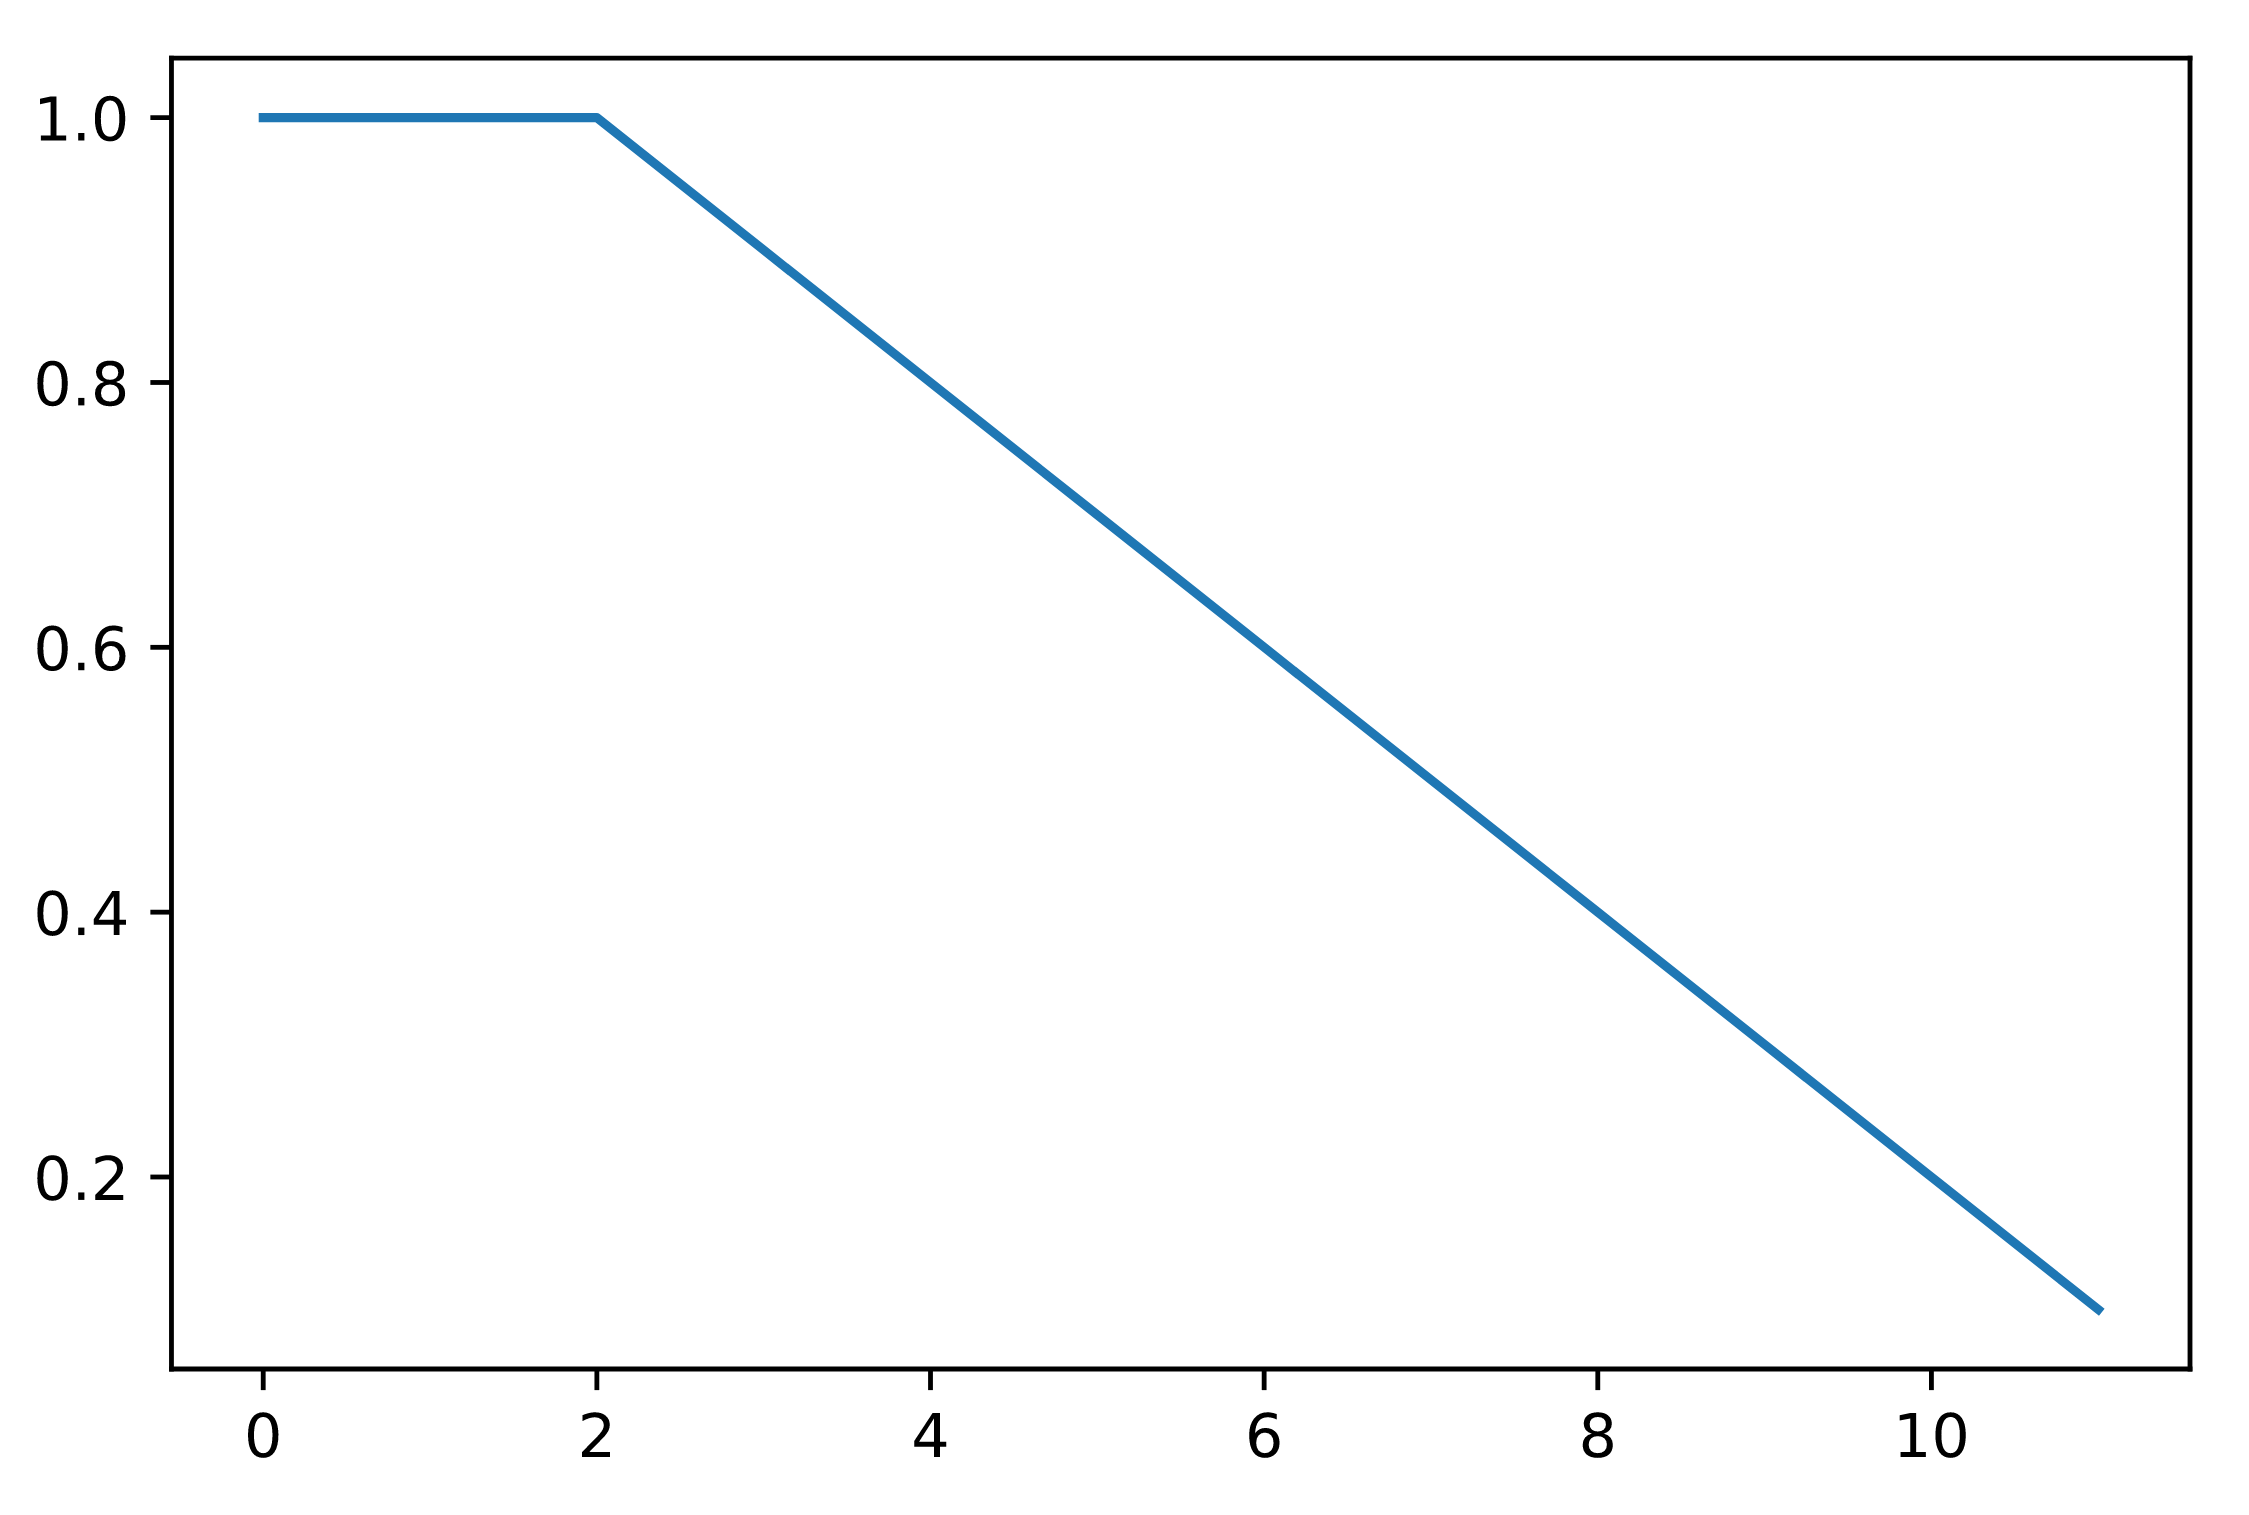
\includegraphics[scale=.0528]{../img/lin}
		\label{fig:lin}
	}
	\subfigure[$\hat\mu_{\text{qlin}}$]
	{
		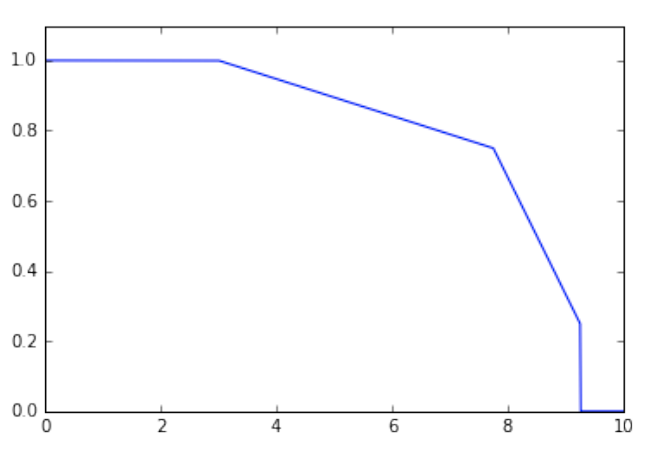
\includegraphics[scale=.18]{../img/qlin}
		\label{fig:qlin}
	}
	\subfigure[$\hat\mu_{\text{exp}}$]
	{
		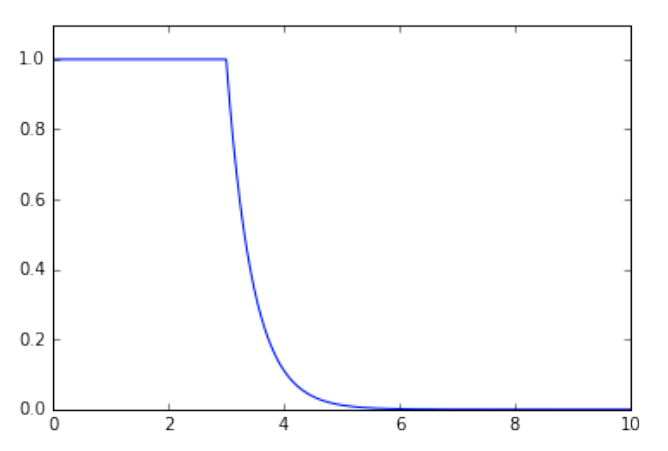
\includegraphics[scale=.18]{../img/exp}
		\label{fig:exp}
	}	
	\caption{Esempio di \emph{fuzzifiers} per un insieme I. L'asse delle ordinate rappresenta il grado di appartenenza e l'asse delle ascisse rappresenta la distanza dalla sfera. Al crescere della distanza diminuisce il grado di appartenenza all'insieme I secondo il \emph{fuzzifier}.}
	\label{fig:fuzzifier}
\end{figure}

%TODO commenta gli esempi di fuzzifier
Un secondo iperparametro che troviamo in \emph{fuzzylearn} è la costante $C$ che compare nella funzione obiettivo:

\[ \min R^2 + C\sum_{i=1}^{n} (\xi_{i} + \tau_{i}) \]

Questa costante rappresenta un iperparametro che definisce il costo dell'errore nella classificazione degli elementi durante la costruzione dell'ipersfera. Questa $ C$ funziona in maniera analoga alla $C$ nelle SVM (Support Vector Machine) \cite{ben_hur}. Tanto più è grande $C$, tanto più sarà elevato il costo dell'errore nel posizionamento delle immagini dei punti dentro o fuori dall'ipersfera. Al contrario, tanto più è piccola $C$, tanto più piccolo sarà il costo dell'errore. 

In Figura \ref{fig:possibilearn_c}, possiamo osservare il ruolo di questo iperparametro al variare del suo valore. La spezzata tratteggiata è una funzione di appartenenza fissata, e sull'asse delle ascisse ci sono i valori di $ x $, colorati in funzione del valore associato da questa funzione. La curva blu è invece la funzione di appartenenza appresa a partire dai punti, per valori diversi dell'iperparametro $ C $. L'errore è quindi legato all'area tra la spezzata e la curva. Si vede come esista un valore di $ C $ che ci permette di ottenere un errore bassissimo (nel grafico a sinistra le due funzioni praticamente sono sovrapposte), e che all'aumentare di $ C $, la funzione tende a diventare binaria e a identificare i dati più significativi per l'insieme (quelli per cui il grado di appartenenza non è nulla). 
%Non mi convince funzione di appartenenza di un insieme
\begin{figure}[h!]
	\centering
	\subfigure[$C = 0.0421$]
	{
		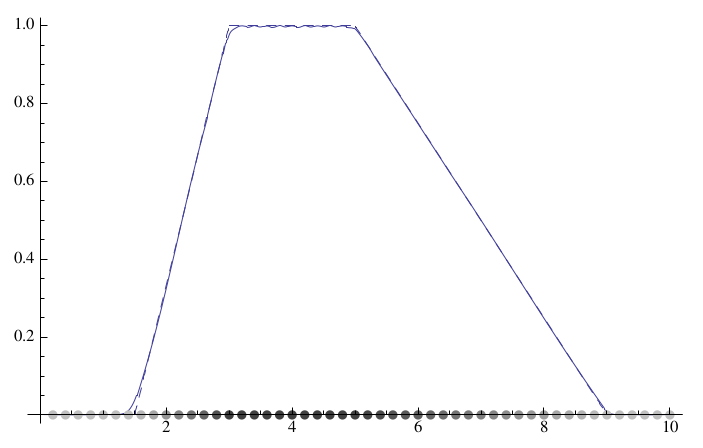
\includegraphics[scale=.18]{../img/possibilearn_c_00421}
	}
	\subfigure[$C = 0.08$]
	{
		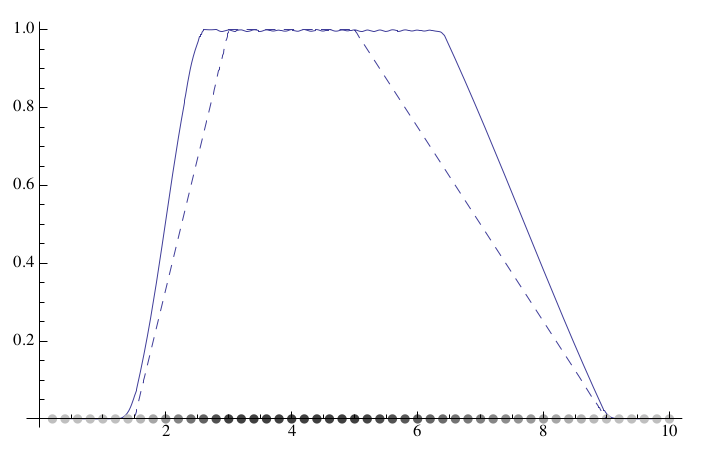
\includegraphics[scale=.18]{../img/possibilearn_c_008}
	}
	\subfigure[$C = 0.15$]
	{
		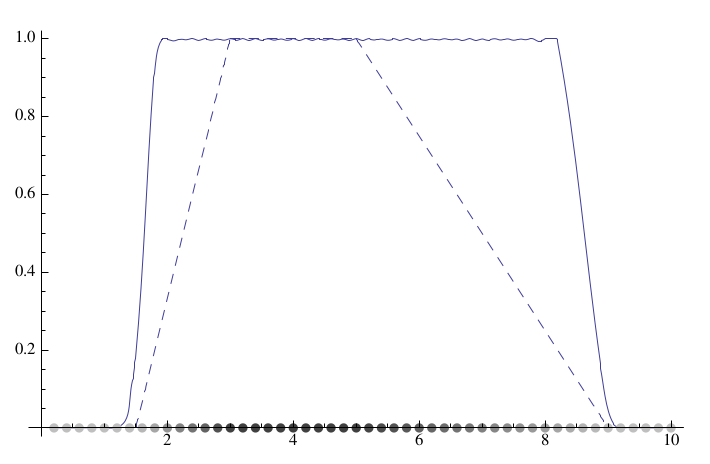
\includegraphics[scale=.18]{../img/possibilearn_c_015}
	}	
	\caption{Nelle figure è mostrato come incrementando $C$ aumenti la sua ``rigidità" aumenta la sua larghezza assomigliando sempre più ad una ``funzione di appartenenza" di un insieme standard.}
	\label{fig:possibilearn_c}
\end{figure}

\begin{figure}[h!]
	\centering
	\subfigure[$\sigma = 0.075$]
	{
		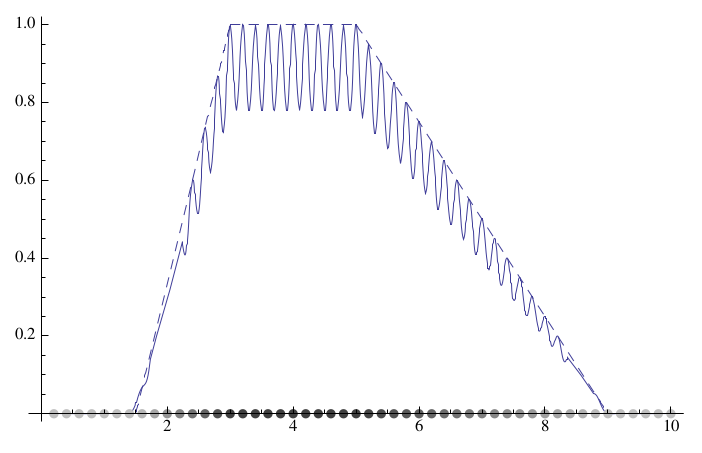
\includegraphics[scale=.18]{../img/possibilearn_sigma_0075}
		\label{fig:first_sub}
	}
	\subfigure[$\sigma = 0.12$]
	{
		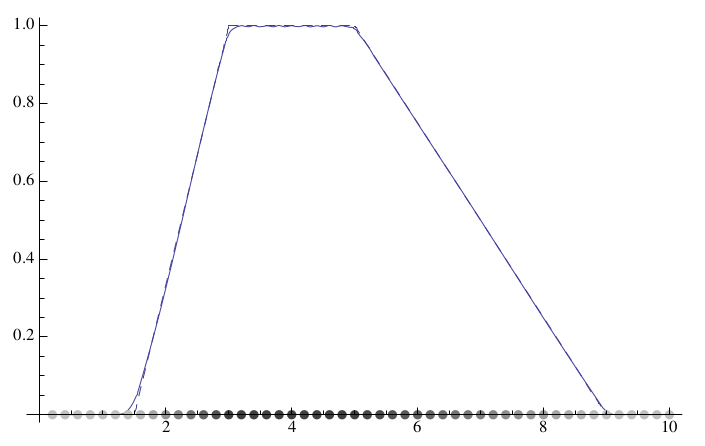
\includegraphics[scale=.18]{../img/possibilearn_sigma_012}
		\label{fig:second_sub}
	}
	\subfigure[$\sigma = 2$]
	{
		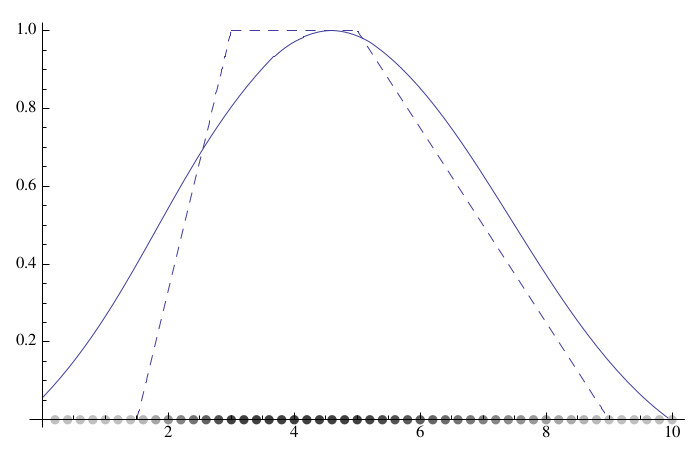
\includegraphics[scale=.18]{../img/possibilearn_sigma_2}
		\label{fig:third_sub}
	}	
	\caption{Nelle figure è mostrato come incrementando $\sigma$ si modifica la forma della funzione di appartenenza.}
	\label{fig:possibilearn_sigma}
\end{figure}

Esiste un ulteriore iperparametro che modifica la funzione di appartenenza, questo è il kernel. Questo iperparametro permette di modificare la forma di $\hat \mu$. Prendendo l'esempio in Figura \ref{fig:possibilearn_sigma} e una funzione kernel gaussiana, vediamo che effetto ha sulla forma della funzione di appartenenza la modifica del parametro $ \sigma $ del kernel.

Ricapitolando, l'algoritmo \emph{fuzzylearn} prevede i tre seguenti iperparametri:
\begin{itemize}
	\item $C$: per determinare il costo degli errori di classificazione in fase di definizione del fuzzy set,
	\item \emph{fuzzifier}: funzione che determina il grado di appartenenza all'insieme fuzzy,
	\item kernel: funzione utile a mappare gli elementi dallo spazio originale ad uno spazio sovra-dimensionato.
\end{itemize}

\chapter{Esperimenti}

In questo capitolo ci concentremo sui risultati ottenuti tramite l'utilizzo di \emph{fuzzylearn} su due diversi dataset di volti: Olivetti faces e AT\&T faces. Descriveremo inoltre tutti i risultati commentandoli e traendo infine delle conclusioni sull'algoritmo utilizzato con le tecniche di riduzione PCA e \emph{t}-SNE.

\section{I dataset}
\subsection{Olivetti dataset}
Olivetti dataset è un dataset di immagini di volti umani. Le immagini sono foto scattate presso AT\&T Laboratories Cambridge tra il 1992 e 1994. Questo dataset è stato messo a disposizione proprio da AT\&T Laboratories Cambridge.
Nel dataset sono presenti 10 immagini per 40 soggetti distinti, ognuna delle quali raffigura quest'ultimo in diverse condizioni di luce, con differenti espressioni facciali (occhi chiusi/aperti, sorriso, ecc.) per un totale di 400 immagini. Ogni immagine è stata quantizzata a 256 livelli di grigio e con una risoluzione pari a 64 x 64. L'immagine è rappresentata da una lista di valori float (compresi tra 0 e 1) di 4096 elementi. Ogni soggetto è rappresentato tramite un numero che va da 0 a 39 che rappresenta l'etichetta di ogni record.

[FIGURA DI HEAD DEL DATASET]


\subsection{AT\&T faces dataset}
Il dataset AT\&T faces, come quello Olivetti, contiene anch'esso immagini raffiguranti 40 soggetti con 10 immagini distinte per ciascuno. Questo dataset, a differenza di Olivetti contiene immagini che sono grandi più del doppio di quelle raffigurate all'iterno del dataset di Olivetti. Ogni immagine a una risoluzione pari a 92 x 112, quindi con 10.304 pixel. Ogni immagine ha 256 livelli di grigio e ritrae soggetti in diverse condizioni, esattamente come Olivetti. Ogni immagine è etichettata da un numero compreso tra 0 e 39 il quale rappresenta il soggetto.[nota: si ringrazia AT\&T Laboratories per i dati messi a disposzione] 

[FIGURA DI HEAD DEL DATASET?]

\section{Valutazione del modello}
Fino ad ora abbiamo visto come si costruiscono i modelli di ML e come possono essere configurati. In questo capitolo ci soffermeremo sulla valutazione di un modello e i relativi iperparametri configurati.

\subsection{Training, Validation e Test set}
Per costruire un modello abbiamo visto che è necessario un dataset su cui basare l'apprendimento. Il dataset che viene usato per la costruzione viene spesso diviso in due sotto-set: \emph{training set} e \emph{test set}.

Il \emph{training set} è il sotto-set di dati utilizzata per allenare il modello. Quindi il modello vede e impara da questo set.

Il \emph{test set} consiste nel set di dati del dataset escluso dal \emph{training set}. Questo set, è utilizzato per valutare l'effettiva accuratezza del modello. 
Il \emph{test set} quindi, viene usato per determinare lo \emph{score} del modello nella generalità dei casi.
% avente la migliore configurazione di iperparametri individuata mediante il \emph{validation set}. Lo score viene determinato analogamente a quanto viene fatto con il \emph{validation set}.

A volte si definisce un terzo sotto-set denominato \emph{validation set}. È un set utilizzato per valutare le prestazioni con una specifica configurazione di iperparametri. Viene utilizzato quindi per una ricerca approfondita della migliore configurazione di questi. Una volta determinata la migliore configurazione del modello, questo viene nuovamente testato nel \emph{test set} per vedere come si comporta effettivamente dopo una più approfondita ricerca dei migliori iperparametri.

\subsection{Cross-validation}
La \emph{cross-validation} è un metodo statistico di valutazione delle performance. Con la \emph{cross-validation} i dati dell'intero dataset vengono partizionati in $k$ gruppi ognuno dei quali è denominato \emph{fold} e dove $k$ rappresenta un numero specificato dall'utente. Quando viene utilizzata questa strategia con un $k$ pari a 5, significa che il dataset sarà diviso in 5 combinazioni differenti in 5 \emph{fold}. Per ogni combinazione possibile un \emph{fold} viene utilizzato come \emph{test set} e gli altri come \emph{training set}. Quindi il modello viene allenato per ogni combinazione data da questa strategia, utilizzando i $k-1$ fold per come \emph{training set} e il restante \emph{fold} come \emph{test set}. In Figura è mostrato uno schema di una \emph{cross-validation} a 5 fold.

[FIGURA DEL LIBRO DELLA CROSS VALIDATION 5.1]

L'utilizzo di questa strategia porta diversi vantaggi. Un primo importante vantaggio è rappresentato dal fatto che l'accuratezza del modello è calcolata sulla media di tutti i valori restituiti da ogni \emph{test set} nelle varie combinazioni dei \emph{fold}. Per capire meglio questo vantaggio, vediamo l'esempio seguente. Supponiamo di essere ``fortunati" e quindi di allenare il modello su un \emph{training set} che contiene solo dati di difficile classificazione. Questo significa che il \emph{test set} probabilmente avrà solamente dei dati molto facili da classificare il che permette al modello di avere prestazioni (non veritiere) molto alte. Al contrario se siamo ``sfortunati" avremo che tutti i dati di difficile classificazione sono all'interno del \emph{test set} e quelli semplici nel \emph{training set}. In questo modo avremo risultati piuttosto bassi.
Con l'utilizzo di \emph{cross-validation} però, la possibilità di avere casi come questi sarà molto bassa proprio perchè verranno usati dati di allenamento sempre diversi per uno stesso modello. Il risultato finale sarà quindi composto dalla media di tutti i risultati delle varie combinazioni.

Un'altro vantaggio corrisponde al fatto che oltre a variare l'utilizzo dei dati di allenamento, varia anche la dimensione di questi. Se utilizziamo 10 \emph{fold} ad esempio, significa che il \emph{test set} sarà definito da un decimo della dimensione totale del dataset. Analogamente se ne utilizziamo 5, il \emph{test set} sarò costituito da un quinto del totale.

La \emph{cross-validation} presenta però un grosso svantaggio nelle performance. Questo perchè maggiore sarà il numero di \emph{fold} e maggiore sarà il tempo richiesto per ottenere un risultato. In altre parole con $k$ \emph{fold} avremo un tempo pari a $k$ volte il tempo necessario ad allenarlo.

\subsection{Grid Search}
Ora che abbiamo capito come avviene e su cosa si basa una buona valutazione del modello possiamo passare al prossimo step: la ricerca del miglior modello.
Cercare il miglior modello significa cercare la migliore configurazione di iperparametri che meglio generalizzano il problema originale. 
\emph{Grid Search} è una tecnica molto usata per la ricerca del miglior iperparametro. Questa tecnica consiste nel provare ogni possibile combinazione di iperparametri di nostro interesse. Consideriamo il caso di \emph{fuzzylearn}. Come abbiamo visto nel capitolo precedente vi sono tre differenti iperparametri che caratterizzano l'algoritmo: \emph{C}, \emph{kernel function}, \emph{fuzzifier}. Supponiamo di voler testare i valori 0.001, 0.1, 1, 1000 per C, un kernel gaussian con sigma pari a .225, .5, 1, 2 per il kernel e Linear fuzzifier, CrispFuzzifier per il fuzzifier. Così facendo abbiamo un totale di $ 4 x 4 x 2 = 32 $ combinazioni differenti di iperparametri.
Iterano tutte le possibili combinazioni su un \emph{training set} e valutandone le prestazioni su un \emph{test set} possiamo quindi trovare quale fra tutte le 32 combinazioni restituisca il valore più alto.

Questa tecnica ha degli svantaggi perchè i risultati ottenuti non sempre sono del tutto veri. Questo succede perchè nel testare le prestazioni delle diverse configurazioni consideriamo \emph{test set} differenti per ognuna di queste. Così facendo i risultati ottenuti si basano tutti sul prorpio test set e questo non ci permette di avere un'unica misura per valutrare le effettive prestazioni.

Per risolvere questo problema si ricorre all'utilizzo del \emph{validation set} che permette quindi di determinare quale possa essere la migliore configurazione e successivamente testarne le effettive prestazioni su dati che non sono stati usati per aggiustare la configurazione. In Figura zzz è mostrata la suddivisione del dataset con l'aggiunta del \emph{validation set}.

[FIGURA DI DATASET IN TRAIN TEST E VALIDATION 5.5]

\subsection{Grid Search con Cross-Validation e Nested Grid Search}
Nei due paragrafi precedenti abbiamo visto quale sia una buona valutazione delle performance del modello e successivamente di come si cerchi efffettivamente una buona configurazione di iperparametri. Queste due tecniche vengono spesso utilizzate insieme per vedere in generale quale sia la migliore combinazione possibile per un modello utilizzando diversi dati di \emph{training} e di \emph{test}.
Quindi quello che viene fatto è, per ogni modello, provare su ogni combinazione di dati per il training e il test come funzione ogni combinazione di iperparametri. Questo consente, quindi, un ulteriore grado di valutazione del modello. Il grosso svantaggio di combinare queste due tecniche consiste nel tempo richiesto per la computazione. Per possibilearn C, sigma, fuzzifier come iperparametri configurabili. Supponendo di provare per C i seguenti valori:
[LISTA DI IPERPARAMETRI DI C]
, per sigma i valori: 
[LISTA DI IPERPARAMETRI DI SIGMA]
e mantendo il \emph{fuzzifier} fisso, otteniamo 5 x 5 = 25 possibili combinazioni mostrate in Figura xxx. 
[TABELLA DI TUTTI LE COMBINAZIONI DEGLI IPERPARAMETRI]
A questo le 25 configurazioni dobbiamo moltiplicalre per il numero di fold che usiamo nella cross validation. Prendendo, ad esempio, 5 fold otteniamo 25 x 5 = 125 diversi modelli da costruire!
È importante quindi utilizzare il Grid Search unito alla Cross-Validation prestando attenzione a quali iperparametri si vogliono confrontare per evitare di non fare computazioni eccessivamente lunghe.

%**************PARLA DI NESTED CROSS VALIDATION**************

\section{I risultati}
In conclusione analizziamo i risultati ottenuti sui dataset Olivetti e AT\&T tramite \emph{fuzzylearn}. Nella ricerca e nello studio di come si comporta \emph{fuzzylearn} nel riconoscimento facciale e di classificazione dei soggetti sono stati usati tre computer per ridurre i costi temporali richiesti dall'allenamento di ogni modello. %La scelta di quale tecnica usare ha richiesto diversi giorni poichè il tempo richiesto dalla computazione era sostanzioso.

Inizialmente è stata costruita un'infrastruttura client-server il cui server godeva di alte performance computazionali. Purtoppo queste non sono state sufficienti in quanto i tempi di calcolo erano troppo lunghi. Quindi la computazione è stata in seguito delegata a tecnologie di Google denominate Google Colaboratory le quali hanno di una maggiore performance computazionale permettendo il risparmio di risorse temporali.

Per il calcolo dei risultati, a livello pratico, è stato usato \emph{python 3.7} come lignuaggio di programmazione il quale rappresenta uno dei più utilizzati linguaggi nell'ambito del ML per la sua comodità e semplicità di utilizzo e perchè sono presenti molte librerie ricche di funzionalità sviluppate proprio in \emph{python}. I pacchetti usati durante questi studi sono stati \emph{scitkit\_learn} per l'elaborazione dei dati e \emph{matplotlib} insieme a \emph{plotly} per la produzione di grafici 2D e 3D. In particolare sono state usate le seguenti librerie/funzionalità:
\begin{itemize}
	\item{\emph{GridSearchCV}: funzione di \emph{scikit\_learn} che, presa una lista di valori per ogni iperparametro, applica su diverse suddivisioni del dataset la combinazione di ognuna di queste per trovare poi quella che definisce il modello con lo score medio più alto (come spiegate in \ref{sec:3.2}),}
	\item{\emph{pre-processing}: libreria di \emph{scikit\_learn} utile ad applicare delle trasformazioni ai dati prima che questi vengano usati per allenare il modello. In particolare \emph{StandardScaler} è una funzione di questa libreria per standardizzare le \emph{feature} e \emph{MinMaxScaler} per adattare a uno specifico intervallo (comune a tutte le \emph{feature}) i singoli valori delle \emph{feature},}
	\item{\emph{PCA}: funzione di \emph{scikit\_learn} che, come si può intendere dal nome, serve ad applicare una riduzione di dimensionalità tramite PCA}
	\item{\emph{TSNE}: funzione di \emph{scikit\_learn} che, come si può intendere dal nome, serve ad applicare una riduzione di dimensionalità tramite TSNE}
\item{\emph{pyplot}: libreria di \emph{matplotlib} che ha avuto un utilizzo speicifico nella produzione di grafici 2D quali grafici di dispersione (o \emph{scatter plot}), grafici di contorno e grafici a linea,}
\item{\emph{express}: libreria di \emph{plotly} per la produzione di grafici tridimensionali come grafici di dispersione 3D e grafici di contorno 3D}
\end{itemize}
Inoltre è stato usato il pacchetto di \emph{fuzzylearn} (disponibile su github all'indirizzo https://github.com/dariomalchiodi/fuzzylearn) il quale contiene il codice per l'utilizzo di \emph{fuzzylearn}. Il modello codificato in questo pacchetto è stato adattato alle librerie di \emph{scikit\_learn} per poterne utilizzare le funzionalità di queste. Nello specifico l'adattamento richiede l'impkementazione delle seguenti funzionalità:
\begin{itemize}
\item{\emph{fit(X, y)}: la funzionalità principale di tutti i modelli di ML. \emph{fit} è utilizzata per allenare un modello sui dati \emph{X} conoscendone le rispettive etichette \emph{y},}
\item{\emph{predict(X)}: contiene l'implementazione per predire la classificazione di ogni elemento di \emph{X}, dove \emph{X} è rappresentato da un vettore di elementi. Nel caso specifico di \emph{fuzzylearn}, \emph{predict} restituisce, per ogni $x$ di \emph{X}, la probabilità (tra 0 e 1) che $x$ appartenga al modello,}
\item{\emph{score(X, y)}: contiene l'implementazione dell'accuratezza di predizione del vettore \emph{X} sapendo che le relative etichette sono \emph{y}. In particolare \emph{fuzzylearn} restituisce uno score pari alla differenza al quadrato della probabilità predetta dal modello e l'effettiva probabilità di appartenenza}
\end{itemize}
Nei prossimi due paragrafi vediamo i risultati ottenuti tramite l'utilizzo delle diverse tecniche di riduzione di dimensionalità PCA e t-SNE. Per ogni tecnica vediamo i risultati ottenuti sia per Olivetti dataset che per AT\&T dataset. Inoltre, durante la descrizione dei risultati vediamo anche l'uso di alcuni degli strumenti sopra citati.

\subsection{Utilizzo metodo di riduzione t-SNE}
In questo paragrafo ci concentriamo sui risultati otteuti applicando una riduzione tramite TSNE a 2 e 3 dimensioni. La scelta di queste dimensioni è dovuta al fatto che t-SNE permette di trasformare uno spazio a n dimensioni in uno spazio più piccolo mantenendo (e quindi focalizzandosi) le distanze tra i punti dello spazio originale. Per questo motivo è stato ritenuto più interessante ridurre le dimensioni originali in due dimensioni proiettabili in uno spazio naturale per farne poi un'analisi a livello qualitativo più immediata. Vediamo quindi la distribuzione dei punti quando vengono ridotti in due dimensioni.

[SCATTER PLOT 2D OLIVETTI E AT\&T]

In Figura [SCATTER PLOT 2D OLIVETTI E AT\&T] sono mostrati i grafici di dispersione per entrambi i dataset dopo aver applicato t-SNE a 2 dimensioni. Analizzando quindi i grafici è piuttosto immediata la distinzione dei vari gruppi rappresentanti ogni soggetto. Partendo da una considerazione del tutto qualitativa e visiva possiamo aspettarci come la costruzione dei modelli, con i giusti iperparametri, ci possa restituire una buona accuratezza nella classificazione dei soggetti.

[SCATTER PLOT 3D OLIVETTI E AT\&T]

Diverso è, il caso riportato in Figura [SCATTER PLOT 3D OLIVETTI E AT\&T] in cui sono mostrati i grafici di dispersione in 3 dimensioni. È facile notare come i cluster siano meno distinguibili rispetto alla proiezione in due dimensioni e quindi è naturale pensare che i risultati di classificazioni su 3 dimensioni siano inferiori rispetto a quelli su dati in 2 dimensioni. In Tabella [TABELLA TSNE OLIVETTI E AT\&T] sono mostrati i rispettivi risultati: le colonne indicano i set su cui è stato testato l'insieme dei modelli mentre le righe indicano la dimensioni di riduzione raggiunte. 

[TABELLA TSNE OLIVETTI E AT\&T]

Con la tabella è stato confermato quanto previsto nelle considerazioni visive fatte sui grafici di dispersione in Figura [SCATTER PLOT 2D OLIVETTI E AT\&T] e in Figura [SCATTER PLOT 3D OLIVETTI E AT\&T]. I risultati ottenuti sono frutto di 10 holdout ripetuti con una dimensione per il \emph{test set} pari al 20\% del totale, di conseguenza il restante 80\% è dedicato al \emph{training set}. 

\subsection{Utilizzo metodo di riduzione PCA}
Ora vediamo come si comporta \emph{fuzzylearn} con i dati ridotti tramite PCA. In questo caso abbiamo considerato un numero maggiore di dimensioni rispetto a t-SNE perchè la logica che sta dietro a questo algoritmo è differente da t-SNE. Come abbiamo già visto nel Capitolo 1, PCA riduce le dimensioni eliminando le caratteristiche che contengono la minor quantità di informazioni. In Figura [PLOT LINE PCA RATIO] vediamo i grafici che mostrano come, la quantità di informazione, decresce al crescere di dimensioni da poter utilizzare. La scelta del numero di dimensioni è partita da un'analisi fatta su questo grafico il quale permette di capire fino a dove ha senso spingersi per cercare di ottenere il maggior numero di informazioni mantenendo la complessità del modello (e quindi il numero di caratteristiche che descrivono ogni osservazione) più bassa possibile.
Con PCA sono state sperimentate le riduzioni a 2, 5, 20, e 50 dimensioni. L'unica riduzione che è possibile analizzare è, naturalmente, quella a due dimensioni. Pertanto in Figura [SCATTER PLOT PCA OLIVETTI E AT\&T] è possibile vedere la distribuzione delle osservazioni nel piano. A differenza di t-SNE, in questi grafici si riesce a distinguere solo qualche piccolo cluster e, oltretutto, facendo fatica. Questo non è un buon segno, infatti come vediamo nei risultati più avanti l'accuratezza di classificazione data dall'insieme dei 40 modelli è decisamente di scarsa qualità. Uno dei motivi per cui la differenza è così marcata tra t-SNE e PCA sta proprio nel fatto che le due tecniche affrontano lo stesso problema, ovvero quello di ridurre le dimensioni, analizzando aspetti totalmente diversi. Mentre t-SNE confronta le distanze tra i punti in un iperspazio, PCA va a selezionare solo le \emph{feature} che mantengono la maggior quantità di informazioni. Ritornando al grafico in Figura [PLOT LINE PCA RATIO] vediamo che utilizzando le prime due dimensioni otteniamo solamente il 30% per Olivetti e il 38% per AT&T. Questo dato rispecchia piuttosto bene la distribuzione del grafico di dispersione proprio perchè con solamente il 30% e il 38% vi è un'alta probabilità che i dati siano mischiati. Quindi vediamo in Tabella [TABELLA PCA OLIVETTI E AT&T] i risultati ottenuti nei due dataset tramite l'utilizzo di PCA.

[TABELLA PCA OLIVETTI E AT\&T]

Nella tabella sopra riportata è infatti possibile notare un certo andamento dei risultati che è direttamente proporzionale al numero di feature utilizzate. Questo segue esattamente quanto scritto sopra: con l'aumentare delle dimensioni aumentano le caratteristiche che descrivono l'oggetto.

\subsection{Analisi conclusiva}
Nell Tabelle [TABELLA TSNE OLIVETTI E AT\&T] e [TABELLA PCA OLIVETTI E AT\&T] abbiamo visto quale sia l'accuratezza fornita da \emph{fuzzylearn} sui dataset Olivetti e AT\&T mediante le due tenciche di riduzione PCA e t-SNE. Da questi risultati si evince che entrambe le tecniche portano a buoni e interessanti risultati con la differenza che gli spazi da considerare sono molto diversi. Con t-SNE abbiamo potuto osservare la sua potenzialità nell'immediatezza visiva di rappresentazione dei dati, il quale è un ottimo strumento per poter fare analisi qualitative dei dati. Con PCA, invece, è stato possibile vedere come la ``qualità", intesa come la quantità di informazioni contenute nei dati, influsica sull'accuratezza dei modelli allenati su di essi. Infine possiamo dire che \emph{fuzzylearn} è un ottimo algoritmo che permette, nel caso specifico di riconoscimento facciale, buone prestazioni a detrimento del tempo richiesto per allenare i modelli. Gli aspetti positivi ricadono, quindi, nella possibilità di rendere i modelli molto ``flessibili" grazie ai diversi iperparametri di cui gode e, quindi, di adattarsi bene a contesti complessi come il riconoscimento di volti in immagini, mentre lo svantaggio principale consiste nel tempo richiesto per l'allenamento del modello.


\begin{thebibliography}{9}
	\bibitem{intro_machine_learning} 
	Andreas C. Müller, Muller Andreas C, Sarah Guido. 
	\textit{Introduction to Machine Learning with Python: A Guide for Data Scientists}. 
	``O'Reilly Media, Inc.", 26 Settembre 2016

	\bibitem{3d_face_recocgnition_pca} 
	Yagnesh Parmar. 
	\textit{3D Face Recognition Using PCA: The Robust Face Recognition System Using Matlab}. 
	Lap Lambert Academic Publishing GmbH KG, 2012

 	\bibitem{image_compression_pca}
	Fred Hohman. \textit{Image Compression via PCA}, \\\texttt{https://fredhohman.com/assets/image\_compression.pdf}

	\bibitem{pattern_recocgnition_pca} 
	Niels da Vitoria Lobo, Takis Kasparis, Michael Georgiopoulos, Fabio Roli, James Kwok, Georgios C. Anagnostopoulos, Marco Loog. \textit{Structural, Syntactic, and Statistical Pattern Recognition}. 
	Springer Science \& Business Media, 24 nov 2008

	\bibitem{data_mining_pca} 
	Djamel A. ZighedJan KomorowskiJan Żytkow. \textit{Principles of Data Mining and Knowledge Discovery}. 
	Springer, Berlin, Heidelberg
	
	\bibitem{fuzzylearn}
	Dario Malchiodi, Witold Pedrycz.
	\textit{Learning Membership Functions for Fuzzy Sets
	through Modified Support Vector Clustering}
	F. Masulli, G. Pasi, and R. Yager (Eds.): WILF 2013, LNAI 8256, pp. 52–59, 2013.
	© Springer International Publishing Switzerland 2013
 
	\bibitem{fuzzylearn_charts}
	Dario Malchiodi, Andrea G. B. Tettamanzi.
	\textit{Predicting the Possibilistic core of OWL Axioms through Modified Support Vector Clustering}
	In SAC 2018: Symposium on Applied Comput-ing , April 9–13, 2018, Pau, France. ACM, New York, NY, USA,8 pages. https://doi.org/10.1145/3167132.31673451
 	
 	\bibitem{towards_data_science}
 	Rushikesh Pupale. \textit{Support Vector Machines(SVM) — An Overview}, \\\texttt{https://towardsdatascience.com/https-medium-com-pupalerushikesh-svm}
 	
 	\bibitem{ben_hur}
	Ben-Hur A., Weston J. (2010) \textit{A User’s Guide to Support Vector Machines}. In: Carugo O., Eisenhaber F. (eds) Data Mining Techniques for the Life Sciences. Methods in Molecular Biology (Methods and Protocols), vol 609. Humana Press
 	
 	
 	\bibitem{fletcher_optimization}
  	R. Fletcher. \textit{Practical Methods of Optimization}, 
  	Copyright © 1987 by John Wiley \& Sons, Ltd
 	
	\bibitem{python_data_science} 
 	Jake VanderPlas. 
 	\textit{Python Data Science Handbook: Essential Tools for Working with Data}. 
 	``O'Reilly Media, Inc.", 6 dicembre 2016

 	\bibitem{ruder}
 	Sebastian Ruder. \textit{An overview of proxy-label approaches for semi-supervised learning}
 	\\\texttt{https://ruder.io/semi-supervised/}
	\bibitem{knuthwebsite} 
	Knuth: Computers and Typesetting,
	\\\texttt{http://www-cs-faculty.stanford.edu/\~{}uno/abcde.html}
\end{thebibliography}

\end{document}


 
